% --------------------------------------------------------------
% This is all preamble stuff that you don't have to worry about.
% Head down to where it says "Start here"
% --------------------------------------------------------------

\documentclass[12pt]{article}

\usepackage[latin1,utf8]{inputenc}
\usepackage[brazil]{babel}

\usepackage[margin=1in]{geometry}
\usepackage{amsmath,amsthm,amssymb}
\usepackage{clrscode3e} % for the pseudocode
\usepackage{graphicx}
\usepackage{float}
\usepackage{framed}
\usepackage{caption}
% for tables
\usepackage{booktabs}
\usepackage[table,xcdraw]{xcolor}
% for the graphs %
\usepackage{tikz}
\usetikzlibrary{trees}
\usetikzlibrary{shapes,snakes}
\usepackage{verbatim}

\usepackage{tabto}

\graphicspath{ {imgs/} }

\newcommand{\N}{\mathbb{N}}
\newcommand{\Z}{\mathbb{Z}}

\newenvironment{theorem}[2][Theorem]{\begin{trivlist}
\item[\hskip \labelsep {\bfseries #1}\hskip \labelsep {\bfseries #2.}]}{\end{trivlist}}
\newenvironment{lemma}[2][Lemma]{\begin{trivlist}
\item[\hskip \labelsep {\bfseries #1}\hskip \labelsep {\bfseries #2.}]}{\end{trivlist}}
\newenvironment{exercise}[2][Exercise]{\begin{trivlist}
\item[\hskip \labelsep {\bfseries #1}\hskip \labelsep {\bfseries #2.}]}{\end{trivlist}}
\newenvironment{reflection}[2][Reflection]{\begin{trivlist}
\item[\hskip \labelsep {\bfseries #1}\hskip \labelsep {\bfseries #2.}]}{\end{trivlist}}
\newenvironment{proposition}[2][Proposition]{\begin{trivlist}
\item[\hskip \labelsep {\bfseries #1}\hskip \labelsep {\bfseries #2.}]}{\end{trivlist}}
\newenvironment{corollary}[2][Corollary]{\begin{trivlist}
\item[\hskip \labelsep {\bfseries #1}\hskip \labelsep {\bfseries #2.}]}{\end{trivlist}}

\newcommand\floor[1]{\big\lfloor#1\big\rfloor}
\newcommand\ceil[1]{\big\lceil#1\big\rceil}
\newcommand\bgfrac[2]{\bigg(\dfrac{#1}{#2}\bigg)}


\begin{document}

\title{MAC 5711 - Análise de Algoritmos}
\author{Rodrigo Augusto Dias Faria\\
Departamento de Ciência da Computação - IME/USP}

\maketitle

\begin{comment}
\begin{center}
\textbf{\large{Lista 1}}
\end{center}
\noindent 1. Lembre-se que lg $n$ denota o logaritmo na base 2 de $n$. Usando a definição de notação $O$, prove que\\[6pt]
(a) $3^n$ não é $O(2^n)$
\\[6pt]
Vamos assumir por contradição que $3^n$ é $O(2^n)$, então podemos assumir que existem as variáveis $c > 0$ e $n_0 > 0$ tal que:
\[ 3^n \leq c 2^n, \forall n \geq n_0 \]
\\[6pt]
Vamos dividir os dois lados por $2^n$:
\begin{align*}
 \frac{3^n}{2^n} & \leq \frac{c 2^n}{2^n}, \forall n \geq n_0 \\
 \frac{3^n}{2^n} & \leq c, \forall n \geq n_0
\end{align*}
\\[6pt]
Note que $3^n > 2^n$ e quando $n \rightarrow \infty$, então $\frac{3^n}{2^n} \rightarrow \infty$, logo podemos concluir que não importa quão grande seja a constante $c$ sempre vai existir algum $n$ suficientemente grande tal que:
\[ 3^n > c 2^n\]
Portanto podemos concluir que $3^n \not \in O(2^n)$. $\square$\\
\\[6pt]
(b) $\log_{10}n$ é $O$(lg $n$)
\\[6pt]
Se existem as constantes $c > 0$ e $n_0 > 0$ tal que:
\[ \log_{10}n \leq c \lg n, \forall n \geq n_0 \]
\\[6pt]
então $\log_{10}n$ é $O$(lg $n$). Veja que uma das propriedades dos logaritmos nos diz que:
\[ \log_c a = \frac{\log_b a}{\log_b c} \]
\\[6pt]
Disso concluimos que:
\[ \log_{10} n = \frac{\lg n}{\lg 10} \]
\\[6pt]
Portanto se fizermos $c = \frac{1}{\lg 10}$ e $n_0 = 1$ temos que 
\[ \log_{10}n \leq \frac{\lg n}{\lg 10}, \forall n \geq 1  \]
\\[6pt]
Portanto podemos concluir que $\log_{10}n = O(\lg n)$. $\square$
\\[6pt]
(c) lg $n$ é $O(\log_{10}n)$
\\[6pt]
Se existem as constantes $c > 0$ e $n_0 > 0$ tal que:
\[ \lg n \leq c \log_{10} n, \forall n \geq n_0 \]
\\[6pt]
Então $\lg n = O(\log_{10} n)$. Note que pela propriedade dos logaritmos mostrada no exercício anterior podemos concluir que:
\[ \lg n = \frac{\log_{10} n}{\log_{10} 2}\]
\\[6pt]
Logo se fizermos $c = \frac{1}{\log_{10} 2}$ e $n_0 = 1$ então teremos:
\[ \lg n \leq \frac{\log_{10} n}{\log_{10} 2}, \forall n \geq 1 \]
\\[6pt]
Portanto podemos concluir que $\lg n = O(\log_{10} n)$. $\square$
\\[12pt]
\noindent 2. Usando a definição de notação $O$, prove que \\[6pt]
(a) $n^2 + 10n + 20 = O(n^2)$ 
\\[6pt]
Se existem as constantes $c > 0$ e $n_0 > 0$, tal que: 
\[ n^2 + 10n + 20 \leq cn^2, \forall n \geq n_0 \]
Então $n^2 + 10n + 20 = O(n^2)$. Note também a seguinte relação:
\[ n^2 + 10n + 20 \leq n^2 + 10n^2 + 20n^2 = 31n^2 \]
Logo se fizermos $c = 31$ e $n_0 = 1$ teremos que:
\[ n^2 + 10n + 20 \leq 31n^2, \forall n \geq 1 \]
Portanto podemos concluir que $n^2 + 10n + 20 = O(n^2)$. $\square$
\\[6pt]
(b) $\lceil n/3 \rceil = O(n)$
\\[6pt]
Se existem as constantes $c > 0$ e $n_0 > 0$ tal que:
\[ \lceil n/3 \rceil \leq cn, \forall n \geq n_0 \]
Então $\lceil n/3 \rceil = O(n)$. Note também a seguinte relação.
\[ \lceil \frac{n}{3} \rceil \leq \frac{n}{3} + 1 \leq \frac{n}{3} + n = \frac{4n}{3}, \forall n \geq 1 \]
Logo se fizermos $c = 4/3$ e $n_0 = 1$, teremos:
\[ \lceil n/3 \rceil \leq \frac{4n}{3}, \forall n \geq 1 \]
Portanto podemos concluir que $\lceil n/3 \rceil = O(n)$. $\square$
\\[6pt]
(c) $\lg n = O(\log_{10} n)$ 
\\[6pt]
Se existem as constantes $c > 0$ e $n_0 > 0$ tal que:
\[ \lg n \leq c \log_{10} n, \forall n \geq n_0 \]
Então $\lg n = O(\log_{10} n)$. Note que pela propriedade dos logaritmos mostrada no exercício 1-(b) podemos concluir que:
\[ \lg n = \frac{\log_{10} n}{\log_{10} 2}\]
Logo se fizermos $c = \frac{1}{\log_{10} 2}$ e $n_0 = 1$ então teremos:
\[ \lg n \leq \frac{\log_{10} n}{\log_{10} 2}, \forall n \geq 1 \]
Portanto podemos concluir que $\lg n = O(\log_{10} n)$. $\square$
\\[6pt]
(d) $n = O(2^n)$
\\[6pt]
Se existem as constantes $c > 0$ e $n_0 > 0$ tal que:
\[ n \leq 2^n, \forall n \geq n_0 \]
Então $n = O(2^n)$. Note trivialmente que se fizermos $c = 1$ e $n_0 = 1$, teremos:
\[ n \leq 2^n, \forall n \geq 1 \]
Portanto podemos concluir que $n = O(2^n)$. $\square$
\\[6pt]
(e) $n/1000$ não é $O(1)$
\\[6pt]
Vamos assumir por contradição que $n/1000 = O(1)$, e portanto que existem as constantes $c > 0$ e $n_0 > 0$ tal que:
\[ n/1000 \leq c, \forall n \geq n_0 \]
Note que quando $n \rightarrow \infty$, então $n/1000 \rightarrow \infty$, portanto não importa quão grande seja $c$, com certeza existe um $n$ suficientemente grande tal que:
\[ n/1000 > c\]
Logo podemos concluir que $n/1000 \not \in O(1)$. $\square$.
\\[6pt]
(f) $n^2/2$ não é $O(n)$
\\[6pt]
Vamos assumir por contradição que $n^2/2 = O(n)$, e portanto que existem as constantes $c > 0$ e $n_0 > 0$ tal que:
\[ n^2/2 \leq  cn, \forall n \geq n_0 \]
Dividindo os dois lados por $n$ teremos:
\begin{align*}
  \frac{n^2}{2n} &\leq \frac{cn}{n}, \forall n \geq n_0 \\
  \frac{n}{2} &\leq c, \forall n \geq n_0
\end{align*}
Note que quando $n \rightarrow \infty$, então $\frac{n}{2} \rightarrow \infty$, portanto não importa quão grande seja $c$ com certeza existe um $n$ suficientemente grande tal que:
\[ n^2/2 > cn \]
Portanto podemos concluir que $n^2/2$ não é $O(n)$. $\square$







\clearpage
\begin{center}
\textbf{\large{Lista 2}}
\end{center}
\noindent 1. Resolva as recorrências abaixo: 
\\[6pt]
(a) $T(n) = 2T(\lfloor n/2 \rfloor) + \Theta(n^2)$ \\
(b) $T(n) = 8T(\lfloor n/2 \rfloor) + \Theta(n^2)$ \\
(c) $T(n) = 2T(\lfloor n/2 \rfloor) + \Theta(n^3)$ 
\\[6pt]
Vamos simplificar a recorrência acima escolhendo a função $n^3$ para representar $\Theta(n^3)$ e vamos também assumir que $n$ é uma pontência de 2 e assim podemos remover o operador chão. Logo podemos simplificar $T(n)$ para:
\[ T(n) = 2T(n/2) + n^3 \]
Vamos encontrar uma formula fechada para recorrência acima pelo metódo da expansão, para isso vamos assumir que $n = 2^k$ e $k = \lg n$.
\begin{align*}
 T(n) &= 2T(\frac{n}{2}) + n^3 \\
 T(\frac{n}{2}) &= 2 \left[ 2T(\frac{n}{2^2}) + \left( \frac{n}{2} \right)^3 \right] + n^3 = 2^2T(\frac{n}{2^2}) + 2 \left( \frac{n}{2} \right)^3 + n^3  \\
 T(\frac{n}{2^2}) &= 2^2 \left[ 2T(\frac{n}{2^3}) + \left( \frac{n}{2^2} \right)^3 \right] + 2 \left(\frac{n}{2^2} \right)^3 + n^3 = 2^3T(\frac{n}{2^3}) + 2^2 \left(\frac{n}{2^2} \right)^3 + 2 \left( \frac{n}{2} \right)^3 + n^3 \\
 T(\frac{n}{2^3}) &= 2^3 \left[ 2T(\frac{n}{2^4}) + \left( \frac{n}{2^2} \right)^3 \right] + 2^2 \left(\frac{n}{2^2} \right)^3 + 2 \left( \frac{n}{2} \right)^3 + n^3 = \\
 \hspace{5mm} &= 2^4T(\frac{n}{2^4}) + 2^3 \left( \frac{n}{2^3} \right)^3 + 2^2 \left(\frac{n}{2^2} \right)^3 + 2 \left( \frac{n}{2} \right)^3 + n^3  
\end{align*}
Note que podemos desenvolver os termos gerados pela função $n^3$ da seguinte maneira:
\begin{align*}
 2^3 \left( \frac{n}{2^3} \right)^3 + 2^2 \left(\frac{n}{2^2} \right)^3 + 2 \left( \frac{n}{2} \right)^3 + n^3 =\\
 2^3 \frac{n^3}{2^9} + 2^2 \frac{n^3}{2^6} + 2 \frac{n^3}{2^3} + n^3 =\\
 \frac{n^3}{2^6} + \frac{n^3}{2^4} + \frac{n^3}{2^2} + n^3  \\
\end{align*}
Por essas expansão podemos supor que esse sumatório até $k$ pode ser da seguinte forma:
\[ \sum_{i=0}^{k-1} \frac{n^3}{2^i} = n^3 \sum_{i=0}^{k-1} \frac{1}{2^{2i}} \]
Logo voltando para a recorrência podemos e considerando que $k = \lg n$ teremos
\begin{align*}
 T(n) &= 2^kT(n/2^k) + n^3 \sum_{i=0}^{k-1} \frac{1}{2^{2i}} \\
 T(n) &= 2^{\lg n}T(n/2^{\lg n}) + n^3 \sum_{i=0}^{\lg n -1} \frac{1}{2^{2i}} \\
 T(n) & = n T(n/n) + n^3 \sum_{i=0}^{\lg n -1} \frac{1}{2^{2i}} \\
 T(n) & = n T(1) + n^3 \sum_{i=0}^{\lg n -1} \frac{1}{2^{2i}} \\
 T(n) & = n + n^3 \sum_{i=0}^{\lg n -1} \frac{1}{2^{2i}} 
\end{align*}
Agora vamos simplificar essa formula fechada resolvendo o somatório. Note que esse somatório é uma serie geometrica de razão $r = 1/4$, logo:
\begin{align*}
 \sum_{i=0}^{\lg n -1} \frac{1}{2^{2i}} &= \frac{(1/4)^{\lg n} - 1}{1/4 - 1} \\
 \sum_{i=0}^{\lg n -1} \frac{1}{2^{2i}} &= \frac{1^{\lg n}/4^{\lg n} - 1}{3/4} \\
 \sum_{i=0}^{\lg n -1} \frac{1}{2^{2i}} &= -\frac{4}{3} \left[ \frac{1}{(2^{\lg n})^2} - 1 \right] \\
 \sum_{i=0}^{\lg n -1} \frac{1}{2^{2i}} &= -\frac{4}{3} \left[ \frac{1}{n^2} - 1 \right] \\
 \sum_{i=0}^{\lg n -1} \frac{1}{2^{2i}} &=  \frac{4}{3} - \frac{4}{3n^2}
\end{align*}
voltando a recorrência teremos:
\begin{align*}
 T(n) &= n + n^3 \left[ \frac{4}{3} - \frac{4}{3n^2} \right] \\
 T(n) &= n + \frac{4n^3}{3} - \frac{4n}{3} \\
 T(n) &= n \left[1 - \frac{4}{3} + \frac{4n^2}{3} \right] \\
 T(n) &= n \left[\frac{4n^2}{3} - \frac{1}{3} \right] \\
 T(n) &= n \left[\frac{4n^2 - 1}{3} \right] 
\end{align*}
Agora vamos provar que a formula fechada acima vale para a recorrência $T(n)$ para isso vamos assumir que $n = 2^k$, portanto a formula fechada em função de $2^k$ será:
\begin{align*}
 T(2^k) &= 2^k \left[\frac{2^{2k}4 - 1}{3} \right] \\
 T(2^k) &= 2^k \left[\frac{2^{2k+2} - 1}{3} \right] 
\end{align*}
Vamos provar por indução em $k$

\begin{itemize}
 \item \textbf{caso base:} Para $k = 0$ teremos:
 \[ T(2^0) = T(1) = 2^0 \left[ \frac{2^{2.0 + 2} - 1}{3} \right] = \frac{2^2 - 1}{3} =  \frac{3}{3} = 1\]
 \item \textbf{Hipótese de indução}: Vamos assumir que a formula abaixo vale para $k > 1$:
 \[ T(2^{k-1}) =  2^{k-1} \left[\frac{2^{2(k-1)+2} - 1}{3} \right] = 2^{k-1} \left[\frac{2^{2k} - 1}{3} \right] \]
 \item \textbf{Prova}: Vamos provar que a formula fechada vale para qualquer $k$:
 \begin{align*}
     T(2^{k}) &=  2 \left[ 2^{k-1} \left[\frac{2^{2k} - 1}{3}  \right] \right] + 2^{3k} \\
     \hspace{3mm} &= 2^{k} \left[\frac{2^{2k} - 1}{3} \right] + 2^{3k} \\
     \hspace{3mm} &= \frac{2^{3k}}{3} - \frac{2^k}{3} + 2^{3k} \\
     \hspace{3mm} &= 2^{3k} \left[ \frac{1}{3} + 1 \right] - \frac{2^k}{3} \\
     \hspace{3mm} &= 2^{3k} \left[ \frac{4}{3} \right] - \frac{2^k}{3} \\
     \hspace{3mm} &=  \frac{2^{3k}2^2}{3}  - \frac{2^k}{3} \\
     \hspace{3mm} &=  \frac{2^{3k + 2} - 2^k}{3} \\
     \hspace{3mm} &=  2^k \left[ \frac{2^{2k + 2} - 1}{3} \right]
 \end{align*}

Logo concluímos que a formula é válida. $\square$
\end{itemize}

Conforme demonstrado no exercício a recorrência $T(n) =  n \left[\frac{4n^2 - 1}{3} \right]$ para n sendo uma potência de 2. Portanto podemos concluír que $T(n) = \Theta(n^3)$. 
\\[6pt]
(d) $T(n) = 7T(\lfloor n/3 \rfloor) + \Theta(n^2)$ \\
(e) $T(n) = 2T(\lfloor 9n/10 \rfloor) + \Theta(n)$ \\
\noindent 2. Escreva um algoritmo que ordena uma lista de n itens dividindo-a em três sublistas de aproximadamente $n/3$ itens, ordenando cada sublista recursivamente e intercalando as três sublistas ordenadas. Analise seu algoritmo concluindo qual é o seu consumo de tempo.\\[6pt]
Para este exercício, devemos efetuar uma alteração no $\proc{Mergesort}$ para a divisão do vetor $A$ em três partições utilizando o $\proc{Merge}$ duas vezes ao final para intercalar as três partes ordenadas em um único vetor.

\begin{codebox}
\Procname{$\proc{Mergesort3}(A, p, r)$}
\li    \If $p < r$
\li         \Then
            $k = \floor{(p + r) / 3}$
\li         $m = k+1 + \floor{(p + r) / 3}$
\li         $\proc{Mergesort3}(A, p, k)$
\li         $\proc{Mergesort3}(A, k + 1, m)$
\li         $\proc{Mergesort3}(A, m + 1, r)$
\li         $\proc{Merge}(A, p, k, m)$
\li         $\proc{Merge}(A, p, m, r)$
            \End
\End
\end{codebox}

\textbf{Consumo de tempo}\\[6pt]
As linhas 1-3 consomem $\Theta(1)$. As linhas 4-5 têm consumo $T(\ceil{n / 3})$ e a linha 6 tem consumo $T(n - \ceil{2n / 3})$, já que a terceira partição não tem tamanho exatamente de $\ceil{n / 3}$. Sabemos que o consumo do $\proc{Merge}$ é $\Theta(n)$, logo:\\
\begin{align*}
T(n) & = T(\ceil{n / 3}) + T(\ceil{n / 3}) + T(n - 2\ceil{n / 3}) + \Theta(n) + \Theta(n) \\
& = 2T(\ceil{n / 3}) + T(\ceil{n / 3}) + \Theta(2n) \\
& = 3T(\ceil{n / 3}) + \Theta(2n)
\end{align*}

Como $\Theta(2n)$ é $\Theta(n)$:\\
\begin{align*}
T(n) & = 3T(\ceil{n / 3}) + \Theta(n)
\end{align*}

Simplificando a recorrência, temos:\\
\begin{eqnarray*}
T(n) = \left\{ \begin{array}{rl} 
 1, &\mbox{ $n = 1$} \\
 3T\bgfrac{n}{3} + n, &\mbox{ $n >= 2 $ potência de 2}
       \end{array} \right.
\end{eqnarray*}

Por expansão:\\
\begin{align*}
T(n) & = 3T\bgfrac{n}{3} + n\\
&= 3 \bigg( 3T\bgfrac{n}{3^2} + \bgfrac{n}{3} \bigg) + n &= 3^2T\bgfrac{n}{3^2} + n + n\\
&= 3^2 \bigg( 3T\bgfrac{n}{3^3} + \bgfrac{n}{3^2} \bigg) + n + n &= 3^3T\bgfrac{n}{3^3} + n + n + n\\
&= ... \\
&= 3^kT\bgfrac{n}{3^k} + kn
\end{align*}

Assumindo $k = \log_3{n}$ e $3^k = n$:\\
\begin{align*}
T(n) &= nT\bgfrac{n}{n} + \log_3{n}\\
&= T(1)n + \log_3{n}(n)\\
&= n + n(\log_3{n})\\
\end{align*}

Portanto, $T(n) = n + n(\log_3{n})$ é $\Theta(n\log{n})$.

\begin{proof}
Prova por indução em k.

\textbf{Base:} para $n = 1$
\begin{align*}
T(1) = 1 = 1 + 1(\log_3{1}) = 1+ 0 = 1
\end{align*}

\textbf{Hipótese de Indução:} Assuma que $T(x) = x + x(\log_3{x})$ vale para $1 >= x < n$\\

\textbf{Passo:} para $n >= 2$
\begin{align*}
T(n) = 3T\bgfrac{n}{3} + n &= 3\bigg( \bgfrac{n}{3} + \bgfrac{n(\log_3{\frac{n}{3}})}{3} \bigg) + n & (\text{por HI})\\
&= 3\bgfrac{n}{3} + 3\bigg( \bgfrac{n}{3}\log_3{\frac{n}{3}}\bigg) + n\\
&= n + n + n\log_3{\frac{n}{3}}\\
&= 2n + n\log_3{n} - n\\
&= n + n\log_3{n}
\end{align*}

Como queríamos demonstrar!

\end{proof}

\clearpage
\begin{center}
\textbf{\large{Lista 3}}
\end{center}

\noindent 2. Qual é o consumo de espaço do QUICKSORT no pior caso?\\[6pt]
A avaliação de um algoritmo quanto ao consumo de espaço está relacionada com a necessidade de alocação de espaço adicional na pilha de recursão.

No pior caso, o QUICKSORT será executado uma vez para cada elemento da lista dada de tamanho $n$, ou seja, teremos $n$ chamadas recursivas.

Isso significa que, com uma lista de $n$ elementos, $n$ novas chamadas serão adicionadas à pilha no pior caso, o que nos leva a uma complexidade de espaço O($n$).\\

\noindent 3. Quando um algoritmo recursivo tem como último comando executado, em algum de seus casos, uma chamada recursiva, tal chamada é denominada recursão de calda (\textit{tail recursion}). Um exemplo de recursão de calda acontece no QUICKSORT.
\begin{codebox}
\Procname{$\proc{Quicksort}(A, p, r)$}
\li     q = \proc{Partition}(A, p, r)
\li     \proc{Quicksort}(A, p, q - 1)
\li     \proc{Quicksort}(A, q + 1, r)
\End
\end{codebox}

Toda recursão de calda pode ser substituída por uma repetição. No caso do $\proc{Quicksort}$, obtemos o seguinte:
\begin{codebox}
\Procname{$\proc{Quicksort}(A, p, r)$}
\li     \While $p < r$
\li         \Do
                $q \gets \proc{Partition}(A, p, r)$
\li             \proc{Quicksort}(A, p, q - 1)
\li             $p \gets q + 1$
            \End
\end{codebox}

Mostre como essa ideia pode ser usada (de uma maneira mais esperta) para melhorar significativamente o consumo de espaço no pior caso do $\proc{Quicksort}$.\\[6pt]
O benefício da utilização do loop ao invés da recursão de cauda é que, geralmente, precisamos de menos memória na pilha para ordenar todos os elementos do vetor $A$, já que a implementação sem a recursão de cauda reusa o ambiente da pilha (variáveis locais, parâmetros, etc) a cada iteração.

A profundidade das chamadas recursivas está relacionada com a ordem em que os elementos se encontram. Se, por exemplo, o vetor $A$ está em ordem decrescente, teremos a execução no pior caso. Isso implica na forma em que cada partição é gerada.

Para ter um resultado ainda mais eficiente, os intervalos podem ser comparados para se certificar de que a maior partição é sempre processada de forma iterativa e a menor de forma recursiva, o que garante a menor profundidade de recursão possível para um determinado vetor de entrada e pivô.
\begin{codebox}
\Procname{$\proc{Half-Tail-Quicksort}(A, p, r)$}
\li     \While $p < r$
\li         \Do
                $q \gets \proc{Partition}(A, p, r)$
\li             \If $(q - p) < (r - q)$
\li                 \Then
                    \proc{Half-Tail-Quicksort}(A, p, q - 1)
\li                 $p \gets q + 1$
\li                 \Else
\li                 \proc{Half-Tail-Quicksort}(A, q + 1, r)
\li                 $r \gets q - 1$
                \End
            \End
\end{codebox}


\noindent 4. Considere o seguinte algoritmo que determina o segundo maior elemento de um vetor $v[1..n]$ com $n>=2$ números positivos distintos.\\[6pt]
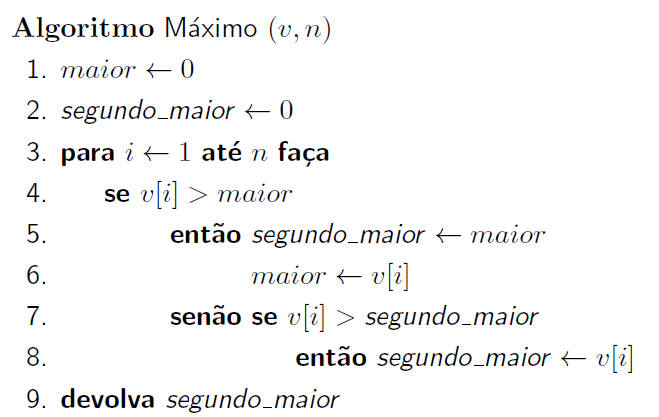
\includegraphics[width=0.6\textwidth]{algo3-4.png}

Suponha que a entrada do algoritmo é uma permutação de 1 a $n$ escolhida uniformemente dentre todas as permutaçõees de 1 a $n$.
Qual é o número esperado de comparações executadas na linha 6 do algoritmo? Qual é o número esperado de atribuições efetuadas na linha 7 do algoritmo?

Vamos calcular $E[X]$ para o algoritmo dado. Seja:\\
A = número de vezes que a linha 5 do algoritmo foi executada\\
B = número de vezes que a linha 8 do algoritmo foi executada\\

X = A + B

\begin{eqnarray*}
X_i = \left\{ \begin{array}{rl} 
 1, &\mbox{ se A ou B} \\
 0, &\mbox{ c.c}
       \end{array} \right.
\end{eqnarray*}

Logo:\\
$E[X_i] = 0 * Pr\{X_i = 0\} + 1 * Pr\{X_i = 1\} = Pr\{X_i = 1\}$\\

Sabemos que a execução da linha 8 depende da avaliação da linha 5, logo:\\
$E[X_i] = Pr\{A\} + (1 - Pr\{A\})*Pr\{B|\bar{A}\}$\\

Como já vimos para a versão original do algoritmo $\proc{Máximo}$ é $Pr\{A\} = \dfrac{1}{i}$.\\
Para a probabilidade de execução da linha 8, temos que:\\
$Pr\{B|\bar{A}\} = \dfrac{1}{1 - i}$\\

Portanto:
\begin{align*}
E[X_i] &= \bgfrac{1}{i} + \bigg(1 - \dfrac{1}{i}\bigg)\bigg(\dfrac{1}{i - 1}\bigg) \\
&= \bgfrac{1}{i} + \bigg(\dfrac{i - 1}{i}\bigg)\bigg(\dfrac{1}{i - 1}\bigg) \\
&= \dfrac{2}{i}
\end{align*}

É fato que a linha 5 sempre será executada na primeira iteração, assumindo que $v[1..n]$ contenha apenas inteiros positivos e $n >= 2$. Logo:
\begin{align*}
E[X_i] &= 1 + \sum_{i=2}^{n} \dfrac{2}{i} = 1 + 2\sum_{i=2}^{n} \dfrac{1}{i}
\end{align*}

\noindent 6. (\textbf{CLRS 8.4-3}) Seja X uma variável aleatória que é igual ao número de caras em duas jogadas de uma moeda justa. Quanto vale $E[X^2]$? Quanto vale $E[X]^2$?\\[6pt]

Como temos dois lançamentos, o espaço amostral é dado por:
\begin{eqnarray*}
S = \{CC, CK, KC, KK\}
\end{eqnarray*}

Sabendo que a $Pr\{X = cara\} = 1/4$, temos que $E[X]$:
\begin{eqnarray*}
  E[X] &=& 2 * \frac{1}{4} + 1 * \frac{1}{4} + 1 * \frac{1}{4} + 0 * \frac{1}{4} \\
  &=& \frac{2 + 1 + 1}{4} + 0 \\
  &=& 1
\end{eqnarray*}

Logo, para $E[X^2]$, temos:
\begin{eqnarray*}
  E[X^2] &=& 2^2 * \frac{1}{4} + 1^2 * \frac{1}{4} + 1^2 * \frac{1}{4} + 0^2 * \frac{1}{4} \\
  &=& \frac{4 + 1 + 1}{4} + 0 \\
  &=& \frac{3}{2}
\end{eqnarray*}

e para $E^2[X]$, temos o produto das esperanças de $X$:
\begin{eqnarray*}
E^2[X] &=& E[X]*E[X] \\
&=& 1 * 1 \\
&=& 1
\end{eqnarray*}
\clearpage

\begin{center}
\textbf{\large{Lista 4}}
\end{center}

\noindent 1. Escreva uma função que recebe um vetor com n letras A’s e B’s e, por meio de trocas, move todos os A’s para o início do vetor. Sua função deve consumir tempo O($n$).\\[6pt]
Resposta\\
\input{l4/q4-02}

\noindent 3. Sejam $X[1..n]$ e $Y[1..n]$ dois vetores, cada um contendo $n$ números ordenados. Escreva um algoritmo O(lg $n$) para encontrar uma das medianas de todos os $2n$ elementos nos vetores $X$ e $Y$.\\[6pt]
Sabemos que a mediana de X e Y está em $i = \floor{q / 2}$ e $j = \floor{s / 2}$, respectivamente. Note que $n = q + s$ é par, e é por isso que nós estamos usando a função \textbf{piso}.

Se $X[i]$ é maior do que $Y[j]$, significa que a mediana global está à esquerda de $X[i]$ e à direita de $Y[j]$. Se $X[i]$ é menor ou igual a $Y[j]$, nós procuramos a mediana à esquerda de $Y[j]$ e à direita de $X[i]$.

A condição de parada dá-se quando $p == q$, o que significa que a mediana global está dentro do vetor $X$. Caso contrário, se $r == s$, a mediana está em $Y$.

O pseudocódigo $\proc{Find-Median}$ mostra a operação descrita acima que, também, é o resultado do exercício 9.3-8 CLRS 3ed.\\

\begin{codebox}
\Procname{$\proc{Find-Median}(X, Y, p, q, r, s)$}
\li \If $p \isequal q$
\li \Comment We have found the median between p, q and r
\li     \Then
            \Return $X[p]$
\li     \ElseIf $r \isequal s$
\li \Comment We have found the median between q, r and s
\li     \Then
            \Return $Y[r]$
        \End
\li $i \gets p + (q - p) / 2$
\li $j = r + (s - r) / 2$
\li \If $X[i] > Y[j]$
\li     \Then
            $q \gets i$
\li         $r \gets j$
\li     \Else
\li         $p \gets i$
\li         $s \gets j$
        \End
\li \Return $\proc{Find-Median}(X, Y, p, q, r, s)$
\End
\end{codebox}
\noindent 4. (\textbf{CLRS 9.3-5}) Para esta questão, vamos dizer que a mediana de um vetor $A[p..r]$ com números inteiros é o valor que ficaria na posição $A[\floor{(p + r)/2}]$ depois que o vetor $A[p..r]$ fosse ordenado.\\
Dado um algoritmo linear “caixa-preta” que devolve a mediana de um vetor, descreva um algoritmo simples, linear, que, dado um vetor $A[p..r]$ de inteiros distintos e um inteiro $k$, devolve o \textit{k-ésimo} mínimo do vetor. (O \textit{k-ésimo} mínimo de um vetor de inteiros distintos é o elemento que estaria na \textit{k-ésima} posição do vetor se ele fosse ordenado.)\\[6pt]

Assumindo que o procedimento $\proc{Median}$ retorna a mediana do vetor $A[p..r]$ em tempo linear, a versão modificada do $\proc{Select}$ abaixo retorna, então, o \textit{k-ésimo} menor elemento de $A[p..r]$.

O algoritmo usa o $\proc{Partition}$ determinístico para pegar um elemento da partição e utilizá-lo como parâmetro de entrada.

\begin{codebox}
\Procname{$\proc{Selection}(A, p, r, k)$}
\li     \If $p == r$
        \Then
\li         \Return $A[p]$
\li     \End
\li     $x \gets \proc{Median}(A, p, r)$
\li     $q \gets \proc{Partition}(x)$
\li     $k \gets q - p + 1$
\li     \If $i == k$
        \Then
\li         \Return $A[q]$
\li     \ElseIf $k < i$
        \Then
\li        \Return $\proc{Selection}(A, p, q - 1, k)$
\li     \Else
\li         \Return $\proc{Selection}(A, p, q + 1, r, k - i)$
\li     \End
\end{codebox}

\noindent 8. (\textbf{CLRS 8.3-2}) Quais dos seguintes algoritmos de ordenação são estáveis: insertionsort, mergesort, heapsort, e quicksort. Descreva uma maneira simples de deixar qualquer algoritmo de ordenação estável. Quanto tempo e/ou espaço adicional a sua estratégia usa?\\[6pt]
Os algoritmos estáveis são o insertionsort e o mergesort (versão do Cormen). Os demais não são estáveis.

Uma forma simples de deixar qualquer algoritmo de ordenação estável é criar um mecanismo de indexação que mantenha a ordem em que os elementos aparecem originalmente, ou seja, basta termos um índice para cada elemento de um vetor de $n$ elementos.

Esse mecanismo necessita de $\Theta(n)$ espaço extra para armazenar os $n$ índices do vetor de $n$ elementos.\\

\clearpage

\begin{center}
\textbf{\large{Lista 5}}
\end{center}


\noindent 1. Desenhe a árvore de decisão para o $\proc{Selectionsort}$ aplicado a $A[1..3]$ com todos os elementos distintos.\\[6pt]
% Set the overall layout of the tree
\tikzstyle{level 1}=[level distance=1.5cm, sibling distance=6cm]
\tikzstyle{level 2}=[level distance=1.5cm, sibling distance=3cm]
\tikzstyle{level 3}=[level distance=1.5cm, sibling distance=3cm]

% Define styles for bags and leafs
\tikzstyle{bag} = [shape=ellipse, draw, align=center,
                   top color=white, bottom color=gray!20]
\tikzstyle{end} = [shape=rectangle, rounded corners, draw, align=center, fill=gray!40]

\begin{tikzpicture}[grow=down]
\node[bag] {1:2}
    child {
        node[bag] {2:3}        
            child {
                node[end]{$\langle 3, 2, 1 \rangle$}
                edge from parent
                node[above] {$\geq$}
            }
            child {
                node[bag] {1:3}
                	child {
                        node[end]{$\langle 3, 1, 2 \rangle$}
                        edge from parent
                        node[above] {$\geq$}
                    }
                	child {
                        node[end]{$\langle 2, 1, 3 \rangle$}
                        edge from parent
                        node[above] {$<$}
                    }
                edge from parent 
                node[above] {$<$}
			}
            edge from parent 
            node[above] {$\geq$}
    }
    child {
        node[bag] {1:3}        
            child {
                node[end]{$\langle 2, 3, 1 \rangle$}
                edge from parent
                node[above] {$\geq$}
            }
            child {
                node[bag] {2:3}
                	child {
                        node[end]{$\langle 1, 3, 2 \rangle$}
                        edge from parent
                        node[above] {$\geq$}
                    }
                	child {
                        node[end]{$\langle 1, 2, 3 \rangle$}
                        edge from parent
                        node[above] {$<$}
                    }
                edge from parent 
                node[above] {$<$}
			}
            edge from parent 
            node[above] {$<$}
    };
\end{tikzpicture}\\

\noindent 2. \textbf{(CLRS 8.1-1)} Qual a menor profundidade (= menor nível) que uma folha pode ter em uma árvore de decisão que descreve um algoritmo de ordenação baseado em comparações?\\[6pt]
\textbf{Resposta:} A menor profundidade da árvore de decisão é, coincidentemente, a cota inferior das alturas de todas as árvores de decisão nas quais aparecem uma folha (uma das $n!$ permutações da entrada).

Também podemos dizer que é o melhor caso em tempo de execução de qualquer algoritmo de ordenação baseado em comparações.

Logo, é o caso em que apenas $n - 1$ comparações são realizadas para ordenar o vetor que ocorre, por exemplo, quando o vetor já está ordenado.\\[12pt]

\noindent 3. Mostre que $lg(n!) \geq \frac{n}{4} lg n$ para $n \geq 4$ sem usar a fórmula de Stirling.\\[6pt]
\textbf{Resposta:} $n!$ pode ser escrito como um produtório:
\begin{align*}
\prod_{k=1}^n k
\end{align*}

Também podemos escrever o produtório como um somatório, pela seguinte identidade (CLRS pp 1061 - 2ed):
\begin{align*}
lg\big(\prod_{k=1}^n k\big) = \sum_{k=1}^n lg(k)
\end{align*}

Logo:
\begin{align*}
lg(n!) = \sum_{k=1}^n lg(k) &= \sum_{k=1}^{\floor{\frac{n}{4}}} lg(k) + \sum_{k=\floor{\frac{n}{4}} + 1}^{2\floor{\frac{n}{4}}} lg(k) + \sum_{k=2\floor{\frac{n}{4}} + 1}^{3\floor{\frac{n}{4}}} lg(k) + \sum_{k=3\floor{\frac{n}{4}} + 1}^{n} lg(k) \\
&\geq \sum_{k=\floor{\frac{n}{4}} + 1}^{n} lg(k) & \text{(descartando 1/4 da soma)} \\
&\geq \sum_{k=\frac{n}{4}}^n lg(\frac{n}{4}) \\
&\geq \frac{n}{4}lg\frac{n}{4} = \frac{n}{4}(lg n - lg 2^2) = \frac{n}{4}(lg n - 2) = \frac{n}{4}lg n - \frac{1}{2}n\\\\
\therefore lg(n!) \geq \frac{n}{4}lg n
\end{align*}


\noindent 4. (\textbf{CLRS 8.1-3}) Mostre que não há algoritmo de ordenação 
baseado em comparações cujo consumo de tempo é linear para pelo menos metade de 
$n!$ permutações de 1 a $n$. O que acontece se trocarmos "metade" por uma 
fração 
de $1/n$? O que acontece se trocarmos "metade" por uma fração de $1/2^n$?
\\ [6pt]
\textbf{Resposta:} Assim como visto em aula uma árvore de decisão pode ser 
utilizada para representar o número de comparações executadas por um algoritmo. 
A árvore de decisão é uma árvore binária onde cada nó não folha é uma 
comparação 
e cada folha é uma permutação de entrada, o caminho da raiz da árvore até uma 
de 
suas folhas mostra a quantidade de comparações executadas para aquela 
permutação, portanto a distância da raiz para a folha mais distânte (altura da 
árvore) reflete o tempo gasto pelo pior caso do algoritmo.
\\[6pt]
Vamos verificar qual a altura da árvore de decisão para saber qual o tempo 
gasto 
no pior caso para pelo menos metade das possíveis permutações $n!/2$. Seja $l$ 
o 
número de folhas do algoritmo e $h$ a altura da árvore, como a árvore de 
decisão 
é uma árvore binária sabemos que ela terá no máximo $2^h$ folhas. Portanto 
temos 
a seguinte relação:
\[ \frac{n!}{2} \leq l \leq 2^h \]
Calculando o logaritmo dos dois lados e sabendo que logaritmo é uma função 
monotonicamente crescente temos que:
\begin{align*}
     \lg 2^h  &\geq  \lg \frac{n!}{2} \\
     h & \geq \lg n! - \lg 2 \\
     h & \geq \lg n! - 1 \\
\end{align*}
Como visto em aula $\lg n! \geq \frac{1}{2} n \lg n$, dessa inequação chegamos 
que $h \geq \lg n! \geq \frac{1}{2} n \lg n$. Disso podemos concluir que $h 
\geq 
\frac{1}{2} n \lg n - 1$, ou seja, mesmo utilizando apenas a metade das 
permutações assintoticamente o algoritmo ótimo gasta $\Omega(n \lg n)$ no pior 
caso.
\\[6pt]
Trocando a "metade" por uma fração $1/n$, podemos utilizar o mesmo raciocínio, 
definindo $l$ como a quantidade de folhas da árvore de decisão e $h$ a altura 
da 
árvore, teremos a seguinte inequação:
\[ \frac{n!}{n} \leq l \leq 2^h \]
Calculando o logaritmo dos dois lados e sabendo que logaritmo é uma função 
monotonicamente crescente temos que:
\begin{align*}
     \lg 2^h  &\geq  \lg \frac{n!}{n} \\
     h & \geq \lg n! - \lg n  \\
     h & \geq n\lg n - \lg n \\
\end{align*}
Note $n\lg n - \lg n = \Theta(n \lg n)$, portanto podemos concluir que para uma 
fração de $1/n$ das permutações também mantem-se gasto de tempo de $\Omega(n 
\lg 
n)$ no pior caso.
\\[6pt]
Trocando a "metade" pela fração de $1/2^n$, podemos utilizar o mesmo raciocínio 
para calcular o pior caso de qualquer algoritmo de ordenação baseada em 
comparações. Seja $l$ o número de folhas e $h$ a altura da árvore teremos a 
seguinte relação:
\[ \frac{n!}{2^n} \leq l \leq 2^h \]
Calculando o logaritmo dos dois lados e sabendo que logaritmo é uma função 
monotonicamente crescente temos que:
\begin{align*}
     \lg 2^h  &\geq  \lg (\frac{n!}{2^n}) \\
     h & \geq \lg (n!) - \lg 2^n \\
     h & \geq n \lg n - n \\
\end{align*}
Note que $n \lg n - n = \Theta(n \lg n)$, portanto da relação acima temos que 
mesmo para a fração de $1/2^n$ de permutações os algoritmos de ordenação que 
utilização comparações consomem tempo $\Omega(n \lg n)$ no pior caso.
\pagebreak

\noindent \textbf{Solução alternativa}
O teorema 8.1 diz que qualquer algoritmo de ordenação por comparação exige $\Omega(n lg n)$ no pior caso.

Estabelecendo uma cota inferior, temos:
\begin{align*}
lg(n!) = lg\big(\prod_{k=1}^n k\big) = \sum_{k=1}^n lg(k) &= \sum_{k=1}^{\floor{\frac{n}{2}}} lg(k) + \sum_{k=\floor{\frac{n}{2}} + 1}^n lg(k) \\
&\geq \sum_{k=\floor{\frac{n}{2}} + 1}^n lg(k) & \text{(descartando 1/2 da soma)} \\
&\geq \sum_{k=\frac{n}{2}}^n lg\bgfrac{n}{2} \\
&\geq \frac{n}{2} lg\bgfrac{n}{2} = \frac{n}{2} (lgn - 1) = \frac{1}{2}nlgn - \frac{1}{2}n = \Omega(n lg n)
\end{align*}

Dizer que o tempo de execução do algoritmo é linear para pelo menos metade das $n!$ permutações, deve valer para $lg\bgfrac{n!}{2}$, o que é absurdo, vejamos:

\begin{align*}
lg\bgfrac{n!}{2} &= lgn! - lg2 = lgn! - 1 \geq \frac{1}{2}nlgn - \frac{1}{2}n - 1
\end{align*}

O mesmo ocorre com $\bgfrac{n!}{n}$ e $\bgfrac{n!}{2^n}$:
\begin{align*}
lg\bgfrac{n!}{n} &= lgn! - lgn \geq \frac{1}{2}nlgn - \frac{1}{2}n - lgn
\end{align*}

\begin{align*}
lg\bgfrac{n!}{2^n} &= lgn! - lg2^n = lgn! - n \geq \frac{1}{2}nlgn - \frac{1}{2}n - n = \frac{1}{2}nlgn - \frac{3}{2}n
\end{align*}

\noindent \textbf{4.1 (CLRS 8.1-4)} Suppose that you are given a sequence of $n$ elements to sort. The input sequence
consists of $n/k$ subsequences, each containing $k$ elements. The elements in a given subsequence are all smaller than the elements in the succeeding subsequence and larger than the elements in the preceding subsequence. Thus, all that is needed to sort the whole sequence of length $n$ is to sort the $k$ elements in each of the $n/k$ subsequences. Show an $\Omega(n lg k)$ lower bound on the number of comparisons needed to solve this variant of the sorting problem. (\textit{Hint:} It is not rigorous to simply combine the lower bounds for the individual subsequences.)

\textbf{Resposta:} A entrada consiste de $n/k$ subsequências, cada uma contendo $k$ elementos, sendo que os elementos da subsequência, digamos $s_i$ são menores que os elementos da subsequência $s_{i+1}$ e maiores que os elementos da subsequência anterior $s_{i-1}$.

O que precisamos fazer para ordenar os $n$ elementos é ordenar os elementos de cada subsequência $s$.

Se pensarmos apenas nos $k$ elementos de uma subsequência, podemos estabelecer uma cota inferior para ordenação:
\begin{align*}
lg(k!) = lg\big(\prod_{i=1}^k i\big) = \sum_{i=1}^k lg(i) &= \sum_{i=1}^{\floor{\frac{k}{2}}} lg(i) + \sum_{i=\floor{\frac{k}{2}} + 1}^k lg(i) \\
&\geq \sum_{i=\floor{\frac{k}{2}} + 1}^k lg(i) & \text{(descartando 1/2 da soma)} \\
&\geq \sum_{i=\frac{k}{2}}^k lg\bgfrac{k}{2} \\
&\geq \frac{k}{2} lg\bgfrac{k}{2} = \frac{k}{2} (lgk - 1) = \frac{1}{2}klgk - \frac{1}{2}k = \Omega(k lg k)
\end{align*}

Como nós temos $n/k$ subsequências, basta combinarmos a cota inferior de cada subsequência com $k$ elementos:
\begin{align*}
\frac{n}{k} \bigg(\frac{1}{2}klgk - \frac{1}{2}k \bigg) = \frac{n}{k} \bigg(\frac{1}{2}klgk \bigg) - \frac{1}{2}n = \frac{1}{2}nlgk - \frac{1}{2}n = \Omega(n lg k)
\end{align*}

\noindent 5. (\textbf{CLRS 8.2-1}) Simule a execução do $\proc{CountingSort}$ 
usando como entrada o vetor:
\[ A[1 \cdots 11] = \langle6, 0, 2, 0, 1, 3, 4, 6, 1, 3, 2\rangle  \]
\\ [6pt]
\textbf{Resposta:} A configuração inicial do algoritmo após o laço inicial será:
\begin{figure}[h]
  \centering
    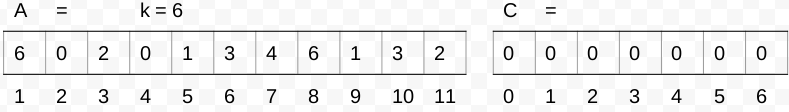
\includegraphics[width=0.8\textwidth]{q5-5-p1}
\end{figure}
\\
O vetor $A$ nunca é alterado, o vetor $C$ é representado abaixo após o final do 
segundo laço (esquerda) e após o final do terceiro laço (direita):
\begin{figure}[h]
  \centering
    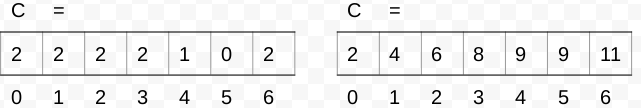
\includegraphics[width=0.8\textwidth]{q5-5-p2}
\end{figure}
\\
O último laço começa pelo com o índice $j = n$ e vai até 1, o vetor B começa 
vázio e vai sendo preenchido até o final do algoritmo. Abaixo segue os estados 
dos vetores $C$ e $B$ no fim das iterações $j = 8, j = 4$ e $j = 1$:
\begin{figure}[h]
  \centering
    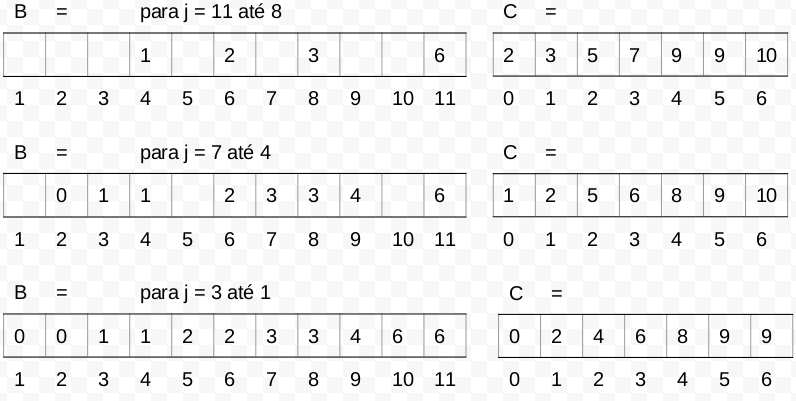
\includegraphics[width=0.8\textwidth]{q5-5-p3}
\end{figure}
\\
Então o algoritmo se encerra mantendo o vetor $B$ ordenado.
\\[12pt]


\noindent 6. (\textbf{CLRS 8.2-2}) Mostre que o \proc{Counting-Sort} é estável.\\[6pt]

\textbf{Resposta:} Vimos em sala que um algoritmo de ordenação é estável se sempre que, inicialmente, $A[i] = A[j]$ para $i < j$, a cópia $A[i]$ termina em uma posição menor do vetor que a cópia $A[j]$. 

O \proc{Counting-Sort} conta quantas vezes um inteiro de $1..k$ aparece em $A[1..n]$ e armazena essa informação no vetor $C$. A próxima iteração faz com que o vetor $C$ tenha a contagem acumulada dos elementos em A. Logo, após essa iteração nós sabemos que $C[i] < C[i + 1]$.

A última iteração ordena efetivamente $A$, copiando seus elementos de $n..1$ para um vetor auxiliar $B$. Como a contagem foi feita na ordem $1..n$ e os valores de $C$ são usados como índices em $B$ e eles são decrementados a cada vez que uma cópia é feita, a ordem relativa em que os elementos aparecem em $A$ é preservada, mesmo no caso onde há repetições, garantindo, assim, a estabilidade do algoritmo.\\[12pt]


\noindent 7. \textbf{(CLRS 8.2-3)} Suponha que o \textbf{para} da linha 7 do $\proc{CountingSort}$ é substituído por 

\begin{codebox}
 \li \For $i \gets 1$ \To $n$ 
\end{codebox}

\noindent Mostre que o $\proc{CountingSort}$ ainda funciona. O algoritmo resultante continua estável?
\\[6pt]
\noindent \textbf{Resposta}: O $\proc{CountingSort}$ continua ordenando o vetor de entrada, o laço substituído ficará:

\begin{codebox}
 \li	\For $j \gets 1$ \To $n$ 
 \li    \Do 
	  $B[C[A[j]]] \gets A[i]$
 \li	  $C[A[i]] \gets C[A[i]] - 1$
	\End
\end{codebox}

Sabemos que o algoritmo não foi modificado antes da linha 7 (do algoritmo original), então o vetor $C$ continua informando, qual a última posição que os elementos de $A$ devem 
ser inseridos, ou seja, $C[i]$ indica onde $A[i]$ deve ser inserido no vetor ordenado $B$, após inseri-lo ele $C[i]$ é decrementando e indicando que o proximo elemento de $A$ que seja igual a $A[i]$ deve ser 
colocado em uma posição anterior assim como o algoritmo dado em aula faz, logo o algoritmo continua ordenado o vetor $A$. Mas com essa alteração o algoritmo
perde informação satelite, ou seja, perde estabilidade, por que ao encontrar um elemento $A[i]$ o mesmo será inserido em $C[A[i]]$ que indica a última posição 
daquele elemento, ao encontrar $A[j] = A[i]$ para $j > i$, o algoritmo ira inseri-lo em $C[A[i]] - 1$, perdendo assim a estabilidade já que $A[i]$ estará 
em uma posição maior que $A[i]$ estará em uma posição maior que $A[j]$ para $A[i] = A[j]$ e $i < j$.

0
\noindent 8. (\textbf{CLRS 8.2-4}) Descreva um algoritmo que, dados $n$ inteiros 
no intervalo de $1$ a $k$, preprocesse sua entrada e então responda em $O(1)$ 
qualquer consulta sobre quantos dos $n$ inteiros dados caem em um intervalo $[a 
\cdots b]$. O preprocessamento efetuado pelo seu algoritmo deve consomir tempo 
$O(n + k)$.
\\[6pt]
\textbf{Resposta}: O algoritmo desenvolvido é baseado no algoritmo de 
\textit{Counting Sort} descrito no livro do Cormen. O algoritmo possuí duas 
rotinas, uma de preprocessamento que devolve um vetor de contagem C e um de 
consulta que retorna a quantidade de elementos conforme o enunciado. O algoritmo 
de preprocessamento abaixo recebe um vetor $A$ de $n$ inteiros qualquer tal que 
seus elementos estão dentro do intervalo $[1 \cdots k]$ e  realiza o 
preprocessamento devolvendo o vetor "$C$" do \textit{counting sort} antes de 
ordena-lo no vetor $B$. Esse vetor possuí o índice do último valor no vetor 
ordenado de cada índice, por exemplo, $C[x] = y$, indica que o último elemento 
$x$ está no índice $y$ do vetor ordenado.

\begin{codebox}
\Procname{$\proc{PreProcessamento}(A, k, n)$}
\li    \For $i \gets 1$ \To $k$
\li    \Do
            $C[i] \gets 0$
       \End
\li    \For $i \gets 1$ \To $n$
\li    \Do
            $C[A[i]] \gets C[A[i]] + 1$
       \End
\li    \For $i \gets 2$ \To $k$
\li    \Do
            $C[i] \gets C[i] + C[i-1]$
       \End
\li    \Return $C$
\End
\end{codebox}
O procedimento $\proc{ContaNoIntervalo}$ recebe o vetor gerado pelo 
$\proc{PreProcessamento}$ e os extremos do intervalo $[a \cdots b]$ e devolve a 
quantidade de elementos do vetor original $A$ que estão dentro desse vetor.
\begin{codebox}
\Procname{$\proc{ContaNoIntervalo}(C, a, b)$}
    \li \If $a \leq 1$
    \li     \Then
            $a' \gets 1$
    \li \Else
            $a' \gets C[a-1] + 1$
        \End
    \li \Return $C[b] - a' + 1$
\End
\end{codebox}
\textbf{Corretude}
\\[6pt]
O procedimento de preprocessamento utiliza o \textit{counting sort} disso 
sabemos que o vetor $C[i]$ contém a quantidade de elementos menores ou iguais a 
$i$ do vetor original, isso implica que o valor de $C[i]$ é a posição do último 
elemento $i$ (não o elemento da posição $i$) do vetor original no vetor 
ordenado, isso implica também que o valor de $C[i-1] + 1$ é a posição do 
primeiro elemento $i$ do vetor original $A$ no vetor ordenado. Disso temos que 
$C[b] - C[a-1] + 1$ é quantidade de elementos com os valores entre $[a \cdots 
b]$ do vetor original. Note que o $if$ do procedimento 
$\proc{ContaNoIntervalo}$, apenas garante que $a-1 \geq 1$ para que não seja 
acessado uma posição fora do vetor $C$, caso isso ocorra consideramos que a 
posição inicial é $1$, note que isso é válido para quando existem valores $1$ em 
$A$ e quando não existem.
\\[6pt]
\textbf{Desempenho}
\\[6pt]
Veja a tabela de gastos em cada linha do procedimento $\proc{PreProcessamento}$:

\begin{table}[H]
\centering
\begin{tabular}{|l|l|}
\hline
Linha                   & Tempo \\ \hline
1 & $\Theta(k)$ \\ \hline
2 & $\Theta(k)$ \\ \hline
3 & $\Theta(n)$ \\ \hline
4 & $\Theta(n)$ \\ \hline
5 & $\Theta(k)$ \\ \hline
6 & $\Theta(k)$ \\ \hline
7 & $\Theta(1)$ \\ \hline
Total & $\Theta(n + k)$ \\ \hline
\end{tabular}
\end{table}
\noindent O procedimento gasta o tempo total $\Theta(n + k)$. O tempo gasto no 
procedimento $\proc{ContaNoIntervalo}$ está expresso na tabela abaixo:
\begin{table}[H]
\centering
\begin{tabular}{|l|l|}
\hline
Linha                   & Tempo \\ \hline
1 & $\Theta(1)$ \\ \hline
2 & $\Theta(1)$ \\ \hline
3 & $\Theta(1)$ \\ \hline
4 & $\Theta(1)$ \\ \hline
Total & $\Theta(1)$ \\ \hline
\end{tabular}
\end{table}
\noindent Portanto o algoritmo gasta tempo $\Theta(n + k)$ para o 
preprocessamento e tempo $\Theta(1)$ para a chamada a contagem dos elementos 
conforme enunciando do exercício.\\[12pt]

\noindent \textbf{8.1 CLRS 8.3-1} Using figure 8.3 as a model, illustrate the operation of RADIX-SORT on the following list of English words: COW, DOG, SEA, RUG, ROW, MOB, BOX, TAB, BAR, EAR, TAR, DIG, BIG, TEA, NOW, FOX.

Basta ordenarmos do dígitos menos significativo ao mais significativo, ou seja, da esquerda para a direita.

\NumTabs{6}
\noindent COW \tab{SEA} \tab{TAB} \tab{BAR} \\
DOG \tab{TEA} \tab{BAR} \tab{BIG} \\
SEA \tab{MOB} \tab{EAR} \tab{BOX} \\
RUG \tab{TAB} \tab{TAR} \tab{COW} \\
ROW \tab{DOG} \tab{SEA} \tab{DIG} \\
MOB \tab{RUG} \tab{TEA} \tab{DOG} \\
BOX \tab{DIG} \tab{DIG} \tab{EAR} \\
TAB \tab{BIG} \tab{BIG} \tab{FOX} \\
BAR \tab{BAR} \tab{MOB} \tab{MOB} \\
EAR \tab{EAR} \tab{DOG} \tab{NOW} \\
TAR \tab{TAR} \tab{COW} \tab{ROW} \\
DIG \tab{COW} \tab{ROW} \tab{RUG} \\
BIG \tab{ROW} \tab{NOW} \tab{SEA} \\
TEA \tab{NOW} \tab{BOX} \tab{TAB} \\
NOW \tab{BOX} \tab{FOX} \tab{TAR} \\
FOX \tab{FOX} \tab{RUG} \tab{TEA} \\[12pt]

\noindent \textbf{8.2 (CLRS 8.3-2)} Which of the following sorting algorithms are stable: \proc{Insertion-Sort}, \proc{Merge-Sort}, \proc{Heap-Sort}, \proc{Quicksort}? Give a simple scheme that makes any sorting algorithm stable. How much additional time and space does your scheme entail?

Os algoritmos estáveis são \proc{Insertion-Sort} e \proc{Merge-Sort}. Podemos manter um outro vetor de tamanho $n$ com a ordem relativa dos elementos originalmente, o que demandaria $\Theta(n)$ espaço adicional e não mudaria o comportamento assintótico do algoritmo.\\[12pt]

\noindent \textbf{9. CLRS 8.3-4} Mostre como ordenar $n$ inteiros no intervalo $0..n^2-1$ em tempo $O(n)$.

Podemos usar o próprio algoritmo \proc{Radix-Sort}. Neste caso, temos $n$ inteiros de 2 dígitos, sendo $k = n$ possíveis valores. Logo:
\begin{align*}
\Theta(d(n + k)) = \Theta(2(n + n)) = \Theta(2n) + \Theta(2n) = \Theta(4n) = \Theta(n)
\end{align*}
\\[12pt]
\noindent 10. Simule a execução do $\proc{BucketSort}$ com o vetor.

\[ A[1..10] = \langle 0.79, 0.13, 0.16, 0.64, 0.39, 0.20, 0.89, 0.53, 0.71, 0.42 \rangle \]
\\[6pt]
\textbf{Resposta:}
\begin{figure}[h]
  \centering
  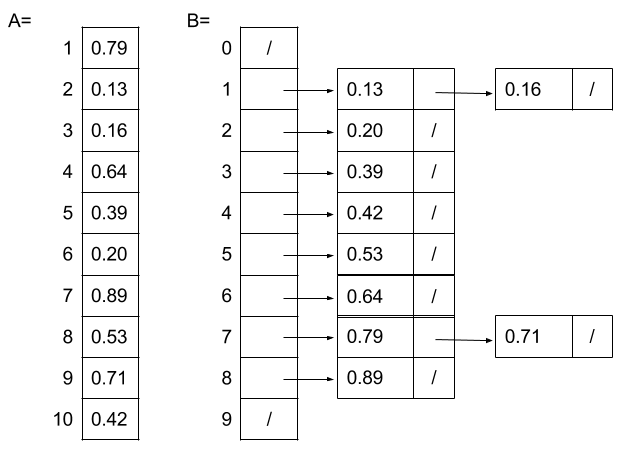
\includegraphics[width=0.7\textwidth]{q5-10}
\end{figure}

\noindent Então cada lista de $B$ é ordenada e concatenada em ordem para gerar o vetor ordenado.
\\[12pt]
\noindent 11. \textbf{(CLRS 8.4-2}: Qual é o consumo de tempo do pior caso para o $\proc{BucketSort}$? Que simples ajuste do algoritmo melhora o seu pior caso para $O(n \lg n)$ e mantem o seu consumo esperado de tempo linear.
\\[6pt]
\noindent \textbf{Resposta:} A resposta do exercício é baseada no algoritmo do livro do CLRS, conforme descrito abaixo:

\begin{codebox}
 \Procname{$\proc{BucketSort}(A)$}
 \li Let $B[0..n-1]$ be a new array
 \li $n \gets \attrib{A}{length}$
 \li \For $i \gets 0$ \To $n-1$
 \li    \Do
	  make $B[i]$ an empty list
	\End
 \li \For $i \gets 1$ \To $n$
 \li	\Do
	  insert $A[i]$ into list $B[\lfloor nA[i] \rfloor]$
	\End
 \li \For $i \gets 0$ \To $n-1$
 \li	\Do
	  sort list $B[i]$ with insertion sort
	\End
 \li concatenate the lists $B[0], B[1], \cdots, B[n-1]$ together in order
\end{codebox}

\noindent O pior caso do $\proc{BucketSort}$ acontence quando a entrada não segue uma distribuição uniforme e todos os itens caem em um único \textit{Bucket}. Como o algoritmo apresentado no CLRS utiliza \textit{insertion sort} para ordenar cada \textit{Bucket} ele gastará tempo $O(n^2)$ no pior caso. Podemos trocar o \textit{insertion sort} pelo $\proc{Mergesort}$ ou $\proc{Heapsort}$ que gastam $O(n \lg n)$ no pior caso. Na prática o \textit{insertion sort} é a melhor opção por que embora gaste tempo $O(n^2)$ \textit{insertion sort} é mais rápido que o $\proc{Mergesort}$ ou o $\proc{Heapsort}$ para vetores pequenos, note que para que o $\proc{BucketSort}$ seja uma boa opção cada \textit{Bucket} tem que ter um número pequeno de elementos.


\noindent \textbf{1. mac338-2011, p2} Suponha que temos que ordenar um vetor com $n$ registros e que a chave de cada registro (o campo que deve ser usado para a ordenação) tem um valor 0 ou 1. Um algoritmo para ordenar esse vetor pode ter um subconjunto das seguintes características:\\[6pt]

\noindent (i) o algoritmo consome tempo $O(n)$;\\[2pt]
(ii) o algoritmo estável;\\[2pt]
(iii) o algoritmo ordena no lugar (ou seja, não usa vetor auxiliar para fazer a ordenação; apenas eventualmente um número constante de variáveis simples).\\[6pt]

\noindent (a) Dê um algoritmo que tenha as características (i) e (ii).\\[2pt]
(b) Dê um algoritmo que tenha as características (i) e (iii).\\[2pt]
(c) Dê um algoritmo que tenha as características (ii) e (iii).\\[12pt]

\noindent \textbf{2. mac338-2011, p2} (Esta questão é uma modificação de um dos exercícios de uma das listas.) Seja $x_1, x_2, \ldots , x_n$ uma sequência de números, onde $n$ é par. Um pareamento de $x_1, x_2, \ldots , x_n$ é uma partição do (multi)conjunto $\{x_1, x_2, \ldots , x_n\}$ em pares. Se P é um pareamento de $x_1, x_2, \ldots , x_n$, então a altura de P é o valor $max\{x_i+x_j : \{x_i, x_j\}$ é um par de $P\}$. Um pareamento de $x_1, x_2, \ldots , x_n$ é ótimo se tem altura mínima.\\[6pt]

\noindent (a) Escreva (em pseudo-código, como nas aulas) um algoritmo que, dado $n$ e um vetor $x[1..n]$ com $n$ números, encontre e devolva um pareamento ótimo de $x[1], x[2], \dots , x[n]$. Seu algoritmo deve
consumir tempo $O(n lg n)$.\\[2pt]
(b) Analise o consumo de tempo do seu algoritmo, concluindo que de fato é $O(n lg n)$.\\[2pt]
(c) Prove que ele de fato produz um pareamento ótimo, ou seja, que nenhum emparelhamento pode ter uma altura menor que a do emparelhamento produzido pelo seu algoritmo.

\textcolor{red}{Tem no gabarito da prova}
\clearpage

\begin{center}
\textbf{\large{Lista 6}}
\end{center}


\noindent 1. (\textbf{CLRS 15.2-1}) Determine a parentização ótima de um produto de cadeia de matrizes cuja sequência de dimensões é $\langle 5, 10, 3, 12, 5, 50, 6 \rangle$.\\[6pt]
\textbf{Resposta:} Como a sequência tem 7 elementos, o valor de $n = 6$. A figura \ref{fig:6.1-1} mostra cada iteração da entrada para geração da matriz $m$ que contém o número mínimo de multiplicações escalares necessário para calcular o produto $A_1..A_n$.

\begin{center}
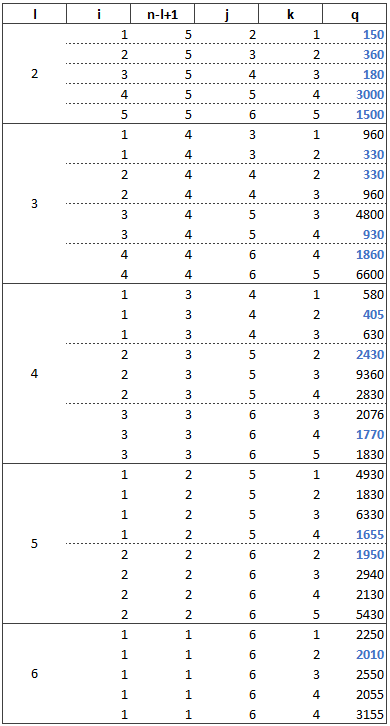
\includegraphics[width=0.6\textwidth]{q6-1-p1.png}
\captionof{figure}{Cálculo do número mínimo de multiplicações escalares}
\label{fig:6.1-1}
\end{center}

Os valores destacados em azul são aqueles menores para uma dada iteração $i, j$ e, consequentemente, são armazenados na matriz $m[i, j]$, como pode ser visto na figura \ref{fig:6.1-2}.
\begin{center}
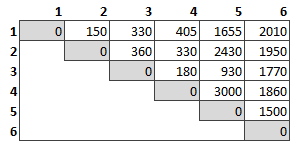
\includegraphics[width=0.4\textwidth]{q6-1-p2.png}
\captionof{figure}{Matriz $m$ preenchida após todas as iterações}
\label{fig:6.1-2}
\end{center}

A figura \ref{fig:6.1-3} mostra uma segunda matriz $s$ utilizada para armazenar o valor de $k$, de forma que possamos rastrear a sequência ótima para multiplicação posteriormente.
\begin{center}
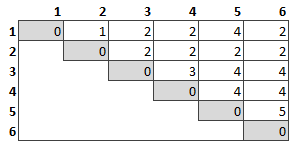
\includegraphics[width=0.4\textwidth]{q6-1-p3.png}
\captionof{figure}{Cálculo do número mínimo de multiplicações escalares}
\label{fig:6.1-3}
\end{center}

Sendo assim, a sequência ótima é $( (A_1 A_2) ((A_3 A_4) (A_5 A_6)) )$.\\[12pt]

\noindent 2. (\textbf{15.2-2}) Adapte o algoritmo dado em aula para que calcule uma matriz $s$ que pode ser usada para determinar uma ordem ótima de multiplicação das matrizes. Dê um algoritmo recursivo que recebe as matrizes $A_1, \ldots, A_n$ em uma matriz tridimensional $A$, recebe a matriz $s$ e índices $i$ e $j$, com $i \leq j$, e faz o produto das matrizes $A_i \ldots A_j$ usando a ordem ótima dada em $s$.\\[6pt]

\textbf{Resposta:} Uma modificação do algoritmo dado no CLRS p. 375 já realiza o procedimento com a matriz $s$, sendo o parâmetro $p$ a sequência com as dimensões das matrizes e $n$ o tamanho de $p - 1$.

\begin{codebox}
\Procname{$\proc{Matrix-Chain-Order}(p, n)$}
\li $m[1..n, 1..n]$ e $s[1..n, 1..n]$ são novas tabelas
\li \For $i \gets 1$ \To $n$
\li \Do
        $m[i, i] \gets 0$
    \End        
\li     \For $l \gets 2$ \To $n$    \Comment l é o tamanho da cadeia
\li     \Do
            \For $i \gets 1$ \To $n - l +1$
\li         \Do
                $j \gets i + l - 1$
\li             $m[i, j] \gets \infty$
\li             \For $k \gets i$ \To $j - 1$
\li             \Do
                    $q = m[i, k] + m[k + 1, j] + p_{i-1} p_k p_j $
\li                 \If $q < m[i, j]$
\li                 \Then
                        $m[i, j] \gets q$
\li                     $s[i, j] \gets k$
                    \End
                \End
            \End
        \End
\li \Return $m, s$
\end{codebox}

Agora, basta calcular o resultado das multiplicações das matrizes na sequência ótima dada por $s$. Quando $i = j$, estamos na base da recursão, ou seja, no ponto em que uma das matrizes de $A$ deve ser retornada para realização da multiplicação. Caso contrário, efetuamos o produto dos pares de matrizes e do resultado do produto dos pares de matrizes que, como é realizado \textit{bottom-up}, termina com uma única matriz quando todas as chamadas recursivas forem concluídas. 

\begin{codebox}
\Procname{$\proc{Matrix-Chain-Multiply}(A, s, i, j)$}
\li \If $i \isequal j$
\li \Then
        \Return $A[i]$
\li \Else
        $a \gets \proc{Matrix-Chain-Multiply}(A, s, i, s[i, j])$
\li     $b \gets \proc{Matrix-Chain-Multiply}(A, s, s[i, j] + 1, j)$
\li     \Return a * b
    \End
\end{codebox}

\noindent 4. (\textbf{15.4-5})  Escreva um algoritmo que, dado $n$ e um vetor $v[1..n]$ de inteiros, determina uma subsequência crescente mais longa de $v$. Seu algoritmo deve consumir tempo $O(n^2)$. Se puder, dê um algoritmo para este problema que consome tempo $O(n lg n)$.

\textbf{Resposta:} Para este exercício, basta utilizarmos os algoritmos \proc{LCS-Length} e \proc{Print-LCS} disponíveis no CLRS 15.4, sendo que o parâmetro $u$ é uma cópia do vetor $v$ ordenado por algum algoritmo de ordenação que, neste caso, usamos o \proc{Quicksort}.

\begin{codebox}
\Procname{$\proc{Build-Longest-Increasing-Subsequence}(v, n)$}
\li $u[1..n]$ vetor auxiliar utilizado para copiar e ordenar $v$
\li \For $i \gets 1$ \To $n$
\li \Do
        $u[i] \gets v[i]$
    \End
\li $\proc{Quicksort}(u, 1, \attrib{u}{length})$
\li	$c, b \gets \proc{LCS-Length}(v, u)$
\li	$\proc{Print-LCS}(b, v, \attrib{v}{length}, \attrib{u}{length})$
\end{codebox}

Como nós queremos encontrar a maior subsequência crescente de $v$, e $u$ é a cópia ordenada de $v$ em ordem crescente, o \proc{LCS-Length} deverá, então, encontrá-la dentre todas as subsequências crescentes dadas por $u$ no vetor original $v$.

A tabela \ref{tbl:6-4-1} mostra o tempo de execução do algoritmo $\proc{Build-Longest-Increasing-Subsequence}$.

\begin{table}[H]
\centering
\begin{tabular}{|l|l|}
\hline
Linha                   & Tempo \\ \hline
1 & $\Theta(1)$ \\ \hline
2 & $\Theta(n)$ \\ \hline
3 & $\Theta(n)$ \\ \hline
4 & $\Theta(n log n)$ \\ \hline
5 & $O(n * n)$ \\ \hline
6 & $O(n + n)$ \\ \hline
Total & $O(n^2 + 2n) + \Theta(n log n) + \Theta(2n) = O(n^2)$ \\ \hline
\end{tabular}
\caption{Tempo de execução}
\label{tbl:6-4-1}
\end{table}

Originalmente, o $\proc{LCS-Length}$ tem tempo de execução em função de $m$ e $n$ ($O(mn)$), porém, como sabemos que $v$ e $u$ têm o mesmo tamanho ($n$), teremos um tempo de execução $O(n^2)$. A mesma analogia vale para o algoritmo $\proc{Print-LCS}$ que é executado na linha 6.\\[12pt]

\noindent 5. Quantas árvores de busca binária existem que guardam 6 diferentes chaves?

\textbf{Resposta:} Vimos em sala que podemos representar 3 nós em 5 árvores de busca binária distintas.

Vamos definir por $t(n)$ o número de diferentes árvores de busca binária para $n$ nós. Sendo assim, o número de diferentes árvores de busca binária que podemos obter deve ter uma raiz, uma subárvore à esquerda com $i$ nós e outra à direita com $n-1-i$ nós para cada $i$, o que nos dá:
\begin{align*}
t(n) = t(0)t(n-1) + t(1)t(n-2) + ... + t(n-1)t(0)
\end{align*}

Logo, podemos estabelecer $t(n)$ como uma recorrência:

\begin{align*}
t(n) = \left\{ \begin{array}{rl} 
 1, &\mbox{ $n = 0$ ou $n = 1$} \\
 \sum_{i=1}^{n} t(i - 1) t(n -  i), &\mbox{ $n > 1 $}
       \end{array} \right.
\end{align*}

A base da recorrência nos diz que há apenas uma árvore de busca binária com nenhum ou um nó.

Sendo assim, para 6 nós, temos 132 árvores de busca binária:
\begin{align*}
t(0) &= 1 \\
t(1) &= t(0)t(0) = 1 \\
t(2) &= t(0)t(1) + t(1)t(0) = 2 \\
t(3) &= t(0)t(2) + t(1)t(1) + t(2)t(0) = 5 \\
t(4) &= t(0)t(3) + t(1)t(2) + t(2)t(1) + t(3)t(0) = 14 \\
t(5) &= t(0)t(4) + t(1)t(3) + t(2)t(2) + t(3)t(1) + t(4)t(0) = 42 \\
t(6) &= t(0)t(5) + t(1)t(4) + t(2)t(3) + t(3)t(2) + t(4)t(1) + t(5)t(0) = 132
\end{align*}

O número de árvores de busca binária também pode ser calculado como o n-\textit{ésimo} número de catalão:
\begin{align*}
C_n = \frac{1}{n + 1}\binom {2n}{n} = \frac{(2n)!}{n!(n + 1)!} = \frac{(2\times6)!}{6!(6 + 1)!} = \frac{12\times11\times10\times9\times8\times7!}{6!7!} = 132
\end{align*}\\[12pt]

\noindent 8. Pode-se generalizar o problema da árvore de busca binária ótima para que inclua na sua descrição uma estimativa do número de buscas mal-sucedidas. Mais concretamente, nessa variante do problema, seriam dados não apenas os números de acessos $a_i$ de cada chave $i$, mas também números $b_i$, para $i = 0, ..., n$, representando uma estimativa do número de buscas mal-sucedidas a elementos entre $i$ e $i+1$ (considere 0 como $-\infty$ e $n-1$ como $+\infty$ para que $b_0$ e $b_n$ sejam o que se espera).
Encontre a recorrência para o custo de uma árvore de busca binária ótima para esta variante do problema. Escreva o algoritmo de programação dinâmica gerado a partir dessa recorrência. Quanto tempo consome o seu algoritmo?\\[6pt]
\textbf{Resposta:} Para generalizarmos o problema da ABB ótima, tal que possamos incluir estimativas de acesso mal sucedidas, vamos pensar em uma ABB que armazena as chaves $k = \langle k_1, k_2, ..., k_n \rangle$ ordenadas e, para cada chave, tenhamos a estimativa do número de acessos a cada elemento de $k$ dado por $a_i$, para todo $i = 1, 2, ..., n$. Essa representação é a que nós já vimos em sala de aula e pode ser vista na figura \ref{fig:6.8-1}.\\

% Set the overall layout of the tree
\tikzstyle{level 1}=[level distance=1.5cm, sibling distance=6cm]
\tikzstyle{level 2}=[level distance=1.5cm, sibling distance=3cm]
\tikzstyle{level 3}=[level distance=1.5cm, sibling distance=2cm]

% Define styles for bags and leafs
\tikzstyle{bag} = [shape=ellipse, draw, align=center,
                   top color=white, bottom color=gray!20]
\tikzstyle{end} = [shape=rectangle, rounded corners, draw, align=center, fill=gray!40]

\begin{figure}[!h]
\centering
\begin{tikzpicture}[grow=down]
\node[bag, label={$a_2$}] {$k_2$}
    child {
        node[bag, label={$a_1$}] {$k_1$}
            edge from parent 
            node[above] {}
    }
    child {
        node[bag, label={$a_4$}] {$k_4$}
            child {
                node[bag, label={$a_3$}] {$k_3$}
                edge from parent 
                node[above] {}
			}
            child {
                node[bag, label={$a_5$}] {$k_5$}
                edge from parent 
                node[above] {}
			}
    };
\end{tikzpicture}
\captionof{figure}{ABB com número de acessos a cada chave}
\label{fig:6.8-1}
\end{figure}

Como temos buscas que são mal sucedidas, ou seja, valores que não estão em $k$, nós devemos estender a ABB de forma a incluir $n+1$ chaves que representam todas essas buscas que, neste caso, denominamos por $q_0, q_1, ..., q_n$. A figura \ref{fig:6.8-2} mostra essa nova representação. Note que, cada nó terminal $k_i$ na estrutura anterior agora recebe novos nós (folhas) que representam as buscas mal sucedidas entre $k_i$ e $k_{i+1}$. Vale ressaltar que, $q_0$ representa todas os valores menores que $k_1$ e $q_n$ representa todos os valores maiores que $k_n$.

Da mesma forma que nas buscas bem sucedidas, temos a estimativa do número de acessos associado a cada chave $q_i$ não encontrada em $k$ que é dado por $b_0, b_1, ..., b_n$.  Por exemplo, se tivéssemos $k = \langle 3, 5, 7, 11, 12\rangle$, se em uma dada ABB $k_3 = 7$ e $k_4 = 11$, o nó terminal $q_3$ representaria os valores não encontrados $\{8, 9, 10\}$.

\begin{figure}[!h]
\centering
\begin{tikzpicture}[grow=down]
\node[bag, label={$a_2$}] {$k_2$}
    child {
        node[bag, label={$a_1$}] {$k_1$}
            child {
                node[end, label={$b_0$}]{$q_0$}
                edge from parent
                node[above] {}
            }
            child {
                node[end, label={$b_1$}]{$q_1$}
                edge from parent
                node[above] {}
            }
            edge from parent 
            node[above] {}
    }
    child {
        node[bag, label={$a_4$}] {$k_4$}
            child {
                node[bag, label={$a_3$}] {$k_3$}
                	child {
                        node[end, label={$b_2$}]{$q_2$}
                        edge from parent
                        node[above] {}
                    }
                	child {
                        node[end, label={$b_3$}]{$q_3$}
                        edge from parent
                        node[above] {}
                    }
                edge from parent 
                node[above] {}
			}
            child {
                node[bag, label={$a_5$}] {$k_5$}
                	child {
                        node[end, label={$b_4$}]{$q_4$}
                        edge from parent
                        node[above] {}
                    }
                	child {
                        node[end, label={$b_5$}]{$q_5$}
                        edge from parent
                        node[above] {}
                    }
                edge from parent 
                node[above] {}
			}
    };
\end{tikzpicture}
\captionof{figure}{ABB estendida adicionando número de buscas mal-sucedidas}
\label{fig:6.8-2}
\end{figure}

Visto isso, podemos definir a \textbf{subestrutura ótima} do problema: se uma ABB é ótima, então as subárvores esquerda e direita também são ótimas. Vale ressaltar que, quando escolhemos uma das chaves, digamos $k_r$ ($i \leq r \leq j$), como a raiz de uma subárvore $k_i, ...,k_j$, a subárvore à esquerda de $k_r$ deve conter as chaves $k_i, ..., k_{r-1}$, bem como as representantes de buscas mal sucedidas $q_{i-1}, ...,q_{r-1}$ e a subárvore à direita de $k_r$ deve conter as chaves $k_{r+1}, ..., k_{j}$ e $q_r, ..., q_j$.

Agora, devemos definir uma solução recursiva para encontrar uma ABB ótima para as chaves $k_1, k_2, ..., k_n$ cujo número esperado de comparações para uma busca bem sucedida $a_1, a_2, ..., a_n$ e o número esperado de comparações para uma busca mal sucedida $b_0, b_1, b_2, ..., b_n$ seja mínimo.

Seja $e[i, j]$ o custo esperado para uma busca em uma ABB ótima com as chaves $i, i+1, ..., j$. Vale a seguinte recorrência para $e[i, j]$:

\begin{align*}
e[i, j] = \left\{\begin{array}{rl}
                    b_{i - 1}, &\mbox{se $i > j$} \\
                    \smash{\displaystyle\min_{i \leq r \leq j}} {e[i, r-1] + e[r+1, j]} + w[i, j], &\mbox{se $i \leq j $}
                \end{array} \right.
\end{align*}

Onde:
\begin{align*}
w[i, j] = \left\{\begin{array}{rl}
                    b_{i - 1}, &\mbox{se $i > j$} \\
                    w[i, j-1] + a_j + b_j, &\mbox{se $i \leq j $}
                \end{array} \right.
\end{align*}

Ou seja, $w[i, j]$ é a soma das estimativas do número de buscas bem e mal sucedidas para um dado $i, j$:
\begin{align*}
w[i, j] = \sum_{l = i}^j a_l + \sum_{l = i-1}^j b_l
\end{align*}

Agora, basta efetuarmos as alterações necessárias no algoritmo dado em sala de aula para calcularmos as matrizes $w$ e $e$. Também vamos armazenar o valor de $r$ em uma matriz $root$, ou seja, qual a raiz foi escolhida para uma determinada subárvore $k_i, ..., k_j$. O algoritmo $\proc{Extended-Optimal-BST}$ mostra o resultado.

\begin{codebox}
\Procname{$\proc{Extended-Optimal-BST}(a, b, n)$}
\li \For $i \gets 1$ \To $n + 1$
\li \Do
        $e[i, i-1] \gets b_{i-1}$
\li     $w[i, i-1] \gets b_{i-1}$
    \End
\li \For $l \gets 1$ \To $n$
\li \Do
        \For $i \gets 1$ \To $n - l + 1$
\li     \Do
            $j \gets i + l - 1$
\li         $w[i, j] \gets w[i, j-1] + a_j + b_j$
\li         $e[i, j] \gets \infty$
\li         \For $r \gets i$ \To $j$
\li         \Do
                $aux \gets e[i, r-1] + e[r+1, j] + w[i, j]$
\li             \If $aux < e[i, j]$
\li             \Then
                    $e[i, j] \gets aux$
\li                 $root[i, j] \gets r$
                \End
            \End
        \End 
    \End
\li \Return $e, root$
\end{codebox}

O custo mínimo da ABB ótima é retornado na posição $e[1, n]$. A tabela \ref{tbl:6-8-1} mostra o tempo de execução do algoritmo $\proc{Extended-Optimal-BST}$. As linhas 4-13 têm 3 \textit{loops} encadeados, que tomam no máximo $n$ iterações cada um, o que nos dá um consumo total $\Theta(n^3)$.

\begin{table}[H]
\centering
\begin{tabular}{|l|l|}
\hline
Linha                   & Tempo \\ \hline
1-3 & $\Theta(n)$ \\ \hline
4-13 & $\Theta(n^3)$ \\ \hline
14 & $\Theta(1)$ \\ \hline
Total & $\Theta(n) + \Theta(n^3) = \Theta(n^3)$ \\ \hline
\end{tabular}
\caption{Tempo de execução}
\label{tbl:6-8-1}
\end{table}

\noindent 10. Escreva uma versão recursiva com memoização do algoritmo descrito em aula para a determinação do custo de uma árvore de busca binária ótima. Quanto tempo consome essa versão do algoritmo para calcular $c(1, n)$?

Basta alterarmos os loops que calculam a tabela $c[i, j]$ por uma versão recursiva memoizada, onde o valor de $c[i, j]$ é retornado, caso já tenha sido calculado. O algoritmo \proc{Memoized-Optimal-BST} mostra essa mudança.

\begin{codebox}
\Procname{$\proc{Memoized-Optimal-BST}(e, n)$}
\li \Comment Seja $s[0..n]$ um novo vetor e $c[0..n][0..n]$ uma nova matriz
\li $s[0] \gets 0$
\li \For $i \gets 1$ \To $n$
\li \Do
        \For $j \gets 0$ \To $n$
\li     \Do
            $c[i, j] \gets \infty$
        \End
\li     $s[i] \gets s[i-1] + e[i]$
    \End
\li \Return $\proc{Lookup-Optimal-BST}(e, s, 1, n)$
\end{codebox}

\begin{codebox}
\Procname{$\proc{Lookup-Optimal-BST}(e, s, i, j)$}
\li \If $c[i, j] < \infty$
\li \Then
        \Return $c[i, j]$
    \End
\li \If $i > j$
\li \Then
        $c[i, j] \gets 0$
\li \Else
        \For $k \gets i+1$ \To $j$
\li     \Do
            $aux \gets \proc{Lookup-Optimal-BST}(e, s, i, k-1) +$
            \Indentmore
\zi         $s[j] - s[i-1] +$
\zi         $\proc{Lookup-Optimal-BST}(e, s, k+1, j)$
            \End
\li         \If $aux < c[i, j]$
\li         \Then
                $c[i, j] \gets aux$
            \End
        \End
    \End
\li \Return $c[1, n]$
\end{codebox}

\textcolor{red}{Falta fazer a análise de tempo}\\[12pt]

\noindent 12. Escreva uma função que recebe como parâmetros um inteiro $n > 0$ e um vetor que armazena uma sequência de $n$ inteiros e devolve o comprimento de uma subsequência crescente da sequência dada de soma máxima. Sua função deve consumir tempo O($n^2$). Modifique a sua função (sem piorar a sua complexidade assintótica) para que ela devolva também uma subsequência crescente da sequência dada de soma máxima.\\[6pt]

\textbf{Resposta:} Assim como no exercício 4, podemos usar uma variação do \proc{LCS-Length} para resolver este problema.

Vamos, então, definir a \textbf{subestrutura ótima} do problema. Seja $X[1..n]$ um vetor com $n$ inteiros e $Y[1..n]$ uma cópia do vetor $X$ ordenado, temos que $Z[1..k]$ é uma subsequência crescente de $X$ de soma máxima, se:

\begin{itemize}
  \item $X[n] = Y[n]$, então $Z[k] = X[n] = Y[n]$ e $Z[1..k-1]$ é subsequência crescente de soma máxima de $X[1..n-1]$ e $Y[1..n-1]$
  \item $X[n] \neq Y[n]$, então $Z[k] \neq X[n]$ implica que $Z[1..k]$ é subsequência crescente de soma máxima de $X[1..n-1]$ e $Y[1..n]$
  \item $X[n] \neq Y[n]$, então $Z[k] \neq Y[n]$ implica que $Z[1..k]$ é subsequência crescente de soma máxima de $X[1..n]$ e $Y[1..n-1]$
\end{itemize}

Logo, percebemos que a subestrutura ótima do problema original não muda. Vamos definir por $c[i, j]$ a soma dos elementos de uma subsequência crescente de soma máxima de $X[1..i]$ e $Y[1..j]$. Vejamos, então, a \textbf{recorrência} para calcular o comprimento da subsequência crescente de soma máxima:
\begin{align*}
c[i, j] = \left\{\begin{array}{rl}
                    0, &\mbox{se $i = 0$ ou $j = 0$} \\
                    c[i-1, j-1] + X[i], &\mbox{se $i, j > 0$ e $X[i] = Y[j]$} \\
                    \smash{\displaystyle\max (c[i, j-1], c[i-1, j])}, &\mbox{se $i, j > 0$ e $X[i] \neq Y[j]$}
                \end{array} \right.
\end{align*}

A diferença para a recorrência original se dá no caso 2, onde o tamanho da LCS era contabilizada. Neste caso, somamos cada elemento de X[i] em uma dada subsequência $X[i..j]$.

O algoritmo \proc{Build-Max-Sum-LCS} efetua, então, o cálculo desejado a partir de um vetor $X[1..n]$. Inicialmente, uma cópia de $X$ é criada e ordenada com um algoritmo de ordenação que, neste caso, utilizamos o \proc{Quicksort}. Posteriormente, chamamos a função \proc{LCS-Max-Sum-Length} que calcula e retorna a matriz $c$ com a soma e a matriz $b$ para que possamos rastrear a subsequência crescente, respectivamente.

Assim que a matriz $b$ é calculada, ela é submetida à rotina $\proc{Get-LCS-Max-Sum}$ que retorna, então, o vetor $Z$ com a subsequência crescente de soma máxima, bem como o tamanho da subsequência.

\begin{codebox}
\Procname{$\proc{Build-Max-Sum-LCS}(X, n)$}
\li $Y[1..n]$ vetor auxiliar utilizado para copiar e ordenar $X$
\li \For $i \gets 1$ \To $n$
\li \Do
        $Y[i] \gets X[i]$
    \End
\li $\proc{Quicksort}(Y, 1, \attrib{Y}{length})$
\li	$c, b \gets \proc{LCS-Max-Sum-Length}(X, Y)$
\li	$Z, l \gets \proc{Get-LCS-Max-Sum}(X, \attrib{X}{length}, b)$
\li \Return Z, l
\end{codebox}

\begin{codebox}
\Procname{$\proc{LCS-Max-Sum-Length}(X, Y)$}
\li $n \gets \attrib{X}{length}$
\li \For $i \gets 0$ \To $n$
\li \Do
        $c[i, 0] \gets 0$
    \End
\li \For $j \gets 1$ \To $n$
\li \Do
        $c[0, j] \gets 0$
    \End
\li \For $i \gets 1$ \To $n$
\li \Do
        \For $j \gets 1$ \To $n$
\li     \Do
            \If $X[i] == Y[j]$
\li         \Then
                $c[i,j] = c[i-1, j-1] + X[i]$
\li             $b[i,j] = "\nwarrow"$
\li         \ElseIf $c[i-1, j] \ge c[i, j-1]$
\li         \Then
                $c[i,j] = c[i-1, j]$
\li             $b[i,j] = "\uparrow"$
\li         \Else
                $c[i,j] = c[i, j-1]$
\li             $b[i,j] = "\leftarrow"$
            \End
        \End
    \End
\li \Return $c, b$
\end{codebox}

A última linha do algoritmo $\proc{Get-LCS-Max-Sum}$ nos devolve a partição de $Z$ que foi preenchida e o tamanho do vetor resultante, ou seja, $n-k$.

\begin{codebox}
\Procname{$\proc{Get-LCS-Max-Sum}(X, n, b)$}
\li $k \gets n$
\li $i \gets n$
\li $j \gets n$
\li \While $i > 0$ and $j > 0$
\li \Do
        \If $b[i,j] == "\nwarrow"$
\li     \Then
            $Z[k] \gets X[i]$
\li         $k \gets k-1$
\li         $i \gets i-1$
\li         $j \gets j-1$
\li     \ElseIf $b[i,j] == "\uparrow"$
\li     \Then
            $i \gets i-1$
\li     \Else
            $j \gets j-1$
        \End     
    \End
\li \Return Z[k..n], n-k
\end{codebox}

Sabemos que o tempo de execução do $\proc{Quicksort}$, $\proc{LCS-Length}$ e $\proc{Get-LCS}$ é $\Theta(n log n)$, $\Theta(mn)$ e $O(m + n)$, respectivamente. As alterações que fizemos em $\proc{LCS-Max-Sum-Length}$ e $\proc{Get-LCS-Max-Sum}$ das versões originais dos respectivos algoritmos não alteram o comportamento assintótico.

Vale lembrar que, o comportamento assintótico do $\proc{LCS-Length}$ e $\proc{Get-LCS}$ são em função de $m$ e $n$ originalmente, como ambos vetores $X$ e $Y$ são de tamanho $n$, o tempo de execução passa a ser em função de $n$, exclusivamente.

Portanto, o consumo de tempo total do \proc{Build-Max-Sum-LCS} é dado na tabela \ref{tbl:6-12-1}:
\begin{table}[H]
\centering
\begin{tabular}{|l|l|}
\hline
Linha                   & Tempo \\ \hline
1 & $\Theta(0)$ \\ \hline
2-3 & $\Theta(n)$ \\ \hline
4 & $\Theta(n log n)$ \\ \hline
5 & $\Theta(n^2)$ \\ \hline
6 & $O(n + n)$ \\ \hline
7 & $\Theta(1)$ \\ \hline
Total & $\Theta(n) + \Theta(n log n) + \Theta(n^2)  + O(2n) = \Theta(n^2)$ \\ \hline
\end{tabular}
\caption{Tempo de execução}
\label{tbl:6-12-1}
\end{table}

\noindent \textbf{13. Problema 15-2 do CLRS (Como imprimir nitidamente)} Considere o problema de imprimir nitidamente um parágrafo em uma impressora. O texto de entrada é uma sequência de $n$ palavras de comprimentos $l_1, l_2, \ldots, l_n$, medidos pelo número de caracteres. Queremos imprimir esse parágrafo com nitidez em uma série de linhas que contêm no máximo $M$ caracteres cada uma. Nosso critério de "nitidez" é dado a seguir. Se uma determinada linha contém palavras de $i$ até $j$, onde $i \leq j$, e deixamos exatamente um espaço entre as palavras, o número de espaços extras no final da linha é $M - j + i - \sum_{k=i}^j l_k$, que deve ser não-negativo para que as palavras caibam na linha. Desejamos minimizar a soma, sobre todas as linhas exceto a última, do cubo do número de espaços extras no final das linhas. Escreva um algoritmo de programação dinâmica para imprimir um parágrafo de $n$ palavras nitidamente em uma impressora. Analise o tempo de execução e os requisitos de espaço do seu algoritmo.

\textbf{Resposta do livro} Note: we will assume that no word is longer than will fit into a line, i.e., $li \leq M$ for all $i$.

First, we'll make some definitions so that we can state the problem more uniformly. Special cases about the last line and worries about whether a sequence of words fits in a line will be handled in these definitions, so that we can forget about them when framing our overall strategy.

Define $extras[i, j] = M - j + i - \sum_{k=i}^j l_k$ to be the number of extra spaces at the end of a line containing words $i$ through $j$. Note that extras may be negative.

Now define the cost of including a line containing words $i$ through $j$ in the sum we want to minimize:

\begin{equation*}
    lc[i, j] =
    \begin{cases}
        \infty & \text{, if } extras[i, j] < 0 \text{ (e.g., words $i, \ldots, j$ don't fit)} \\
        0 & \text{, if } j=n \text{ and } extras[i, j] \geq 0 \text{ (last line costs 0)} \\
        extras[i, j]^3 & \text{, otherwise}
    \end{cases}
\end{equation*}

By making the line cost infinite when the words don't fit on it, we prevent such an arrangement from being part of a minimal sum, and by making the cost 0 for the last line (if the words fit), we prevent the arrangement of the last line from influencing the sum being minimized.

We want to minimize the sum of $lc$ over all lines of the paragraph.

Our subproblems are how to optimally arrange words $1, \ldots, j$, where $j = 1,\ldots, n$.

Consider an optimal arrangement of words $1,\ldots, j$. Suppose we know that the last line, which ends in word $j$, begins with word $i$. The preceding lines, therefore, contain words $1,\ldots,i - 1$. In fact, they must contain an optimal arrangement of words $1,\ldots,i - 1$. (Insert your favorite cut-and-paste argument here.)

Let $c[j]$ be the cost of an optimal arrangement of words 1,\ldots, j. If we know that the last line contains words $i,\ldots, j$, then $c[j] = c[i - 1] + lc[i, j]$. As a base case, when we're computing $c[1]$, we need $c[0]$. If we set $c[0] = 0$, then $c[1] = lc[1, 1]$, which is what we want.

But of course we have to figure out which word begins the last line for the subproblem of words $1,\ldots, j$. So we try all possibilities for word $i$, and we pick the one that gives the lowest cost. Here, $i$ ranges from 1 to $j$. Thus, we can define $c[j]$ recursively by

\begin{equation*}
    c[j] =
    \begin{cases}
        0 & \text{, if } j = 0 \\
        \smash{\displaystyle\min_{1 \leq i \leq j}} (c[i - 1] + lc[i, j]) & \text{, if } j > 0
    \end{cases}
\end{equation*}

Note that the way we defined $lc$ ensures that:

\begin{itemize}
\item all choices made will fit on the line (since an arrangement with $lc = \infty$ cannot be chosen as the minimum), and

\item the cost of putting words $i,\ldots, j$ on the last line will not be 0 unless this really is the last line of the paragraph ($j = n$) or words $i \ldots j$ fill the entire line.
\end{itemize}

We can compute a table of $c$ values from left to right, since each value depends only on earlier values. To keep track of what words go on what lines, we can keep a parallel $p$ table that points to where each $c$ value came from. When $c[j]$ is computed, if $c[j]$ is based on the value of $c[k - 1]$, set $p[j] = k$. Then after $c[n]$ is computed, we can trace the pointers to see where to break the lines. The last line starts at word $p[n]$ and goes through word $n$. The previous line starts at word $p[p[n]]$ and goes through word $p[n] - 1$, etc.

In pseudocode, here's how we construct the tables:
\begin{align}
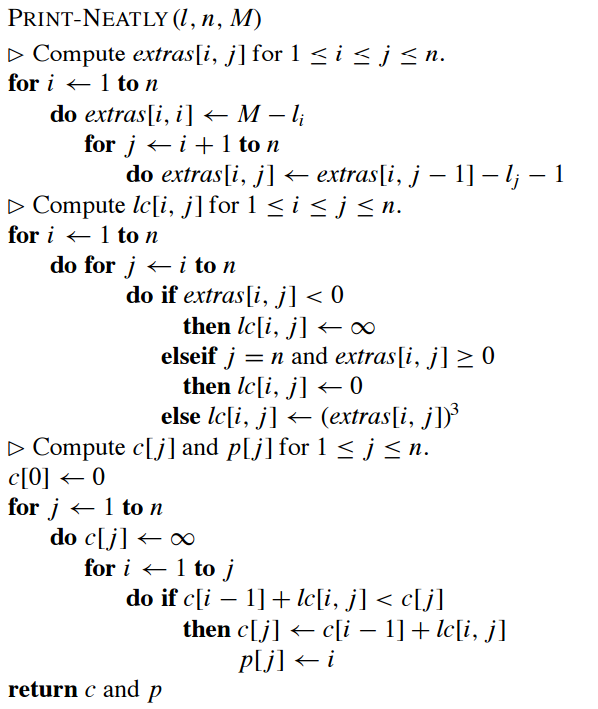
\includegraphics[width=0.65\textwidth]{q6-13-p1.png}
\end{align}

Quite clearly the time and space are $\Theta(n^2)$, but we can get both down to $\Theta(nM)$ (at most \ceil{M/2} words can fit on a line). The space can even further for $\Theta(n)$.

Here's how we print which words are on which line. The printed output of $\proc{Give-Lines}(p, j)$ is a sequence of triples $(k, i, j)$, indicating that words $i, \ldots , j$ are printed on line $k$. The return value is the line number $k$.

\begin{align}
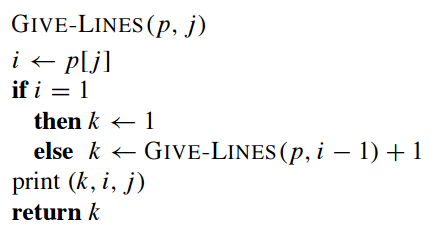
\includegraphics[width=0.5\textwidth]{q6-13-p2.png}
\end{align}

The initial call is $\proc{Give-Lines}(p, n)$. Since the value of $j$ decreases in each recursive call, $\proc{Give-Lines}$ takes a total of $O(n)$ time.\\[12pt]

\noindent \textbf{14. Problema 14-4 do CLRS} (Planejando uma festa da empresa) 
O professor Stewart presta consultoria ao presidente de uma corporação que 
está planejando uma festa da empresa. A empresa tem uma estrutura hierárquica; 
isto é, a relação de supervisores forma uma árvore com raiz no presidente. O 
pessoal do escritório classificou cada funcionário com uma avaliação de 
sociabilidade, que é um número real. Para tornar a festa divertida para todos 
os partocipantes, o presidente não deseja que um funcionário e seu supervisor 
imediato participem.
\\[6pt]
\noindent O professor Stewart recebe uma árvore que descreve a estrutura 
hierárquica da corporação, usando a representação de filho da esquerda, irmão 
da direita, usanda para armazenamento de árvores enraizadas (olhe na seção 
10.4 se precisar). Cada nó da árvore contém além dos ponteiros, o nome de um 
funcionário e a ordem de sociabilidade desse funcionário. Escreva um algoritmo 
para compor a lista de convidados que maximize a soma das avaliações de 
sociabilidade dos convidados. Analise o tempo de execução do seu algoritmo.
\\[6pt]
\noindent \textbf{Resposta: } Vamos resolver esse problema com a técnica de 
programação dinâmica.
\\[6pt]
\noindent \textbf{Sub-estrutura ótima}: Seja $T$ a árvore hierarquica da 
empresa, sabemos que dado a solução ótima $S$ que maximiza a soma de 
sociabilidade da empresa, se a raiz de $T$ pertece a essa solução $S$ a 
sociabilidade dessa solução é a soma da sociabilidade do presidente (raiz da 
árvore) e das soluções ótimas das subárvores enraizadas em seus subordinados 
diretamente, note que seus subordinados não podem ser convidados. Se o 
presidente não pertence a solução ótima desse problema então a sociabilidade da 
solução ótima é a soma das sociabilidades das soluções ótimas das subárvores 
enraizadas em seus subordinados direitos. \textbf{Prova:} Vamos assumir por 
contradição que na solução ótima, dado as subárvores enraizadas nos 
subordinados diretos do presidente exista uma delas que não seja ótima, então 
com certeza podemos trocar essa subárvore que não é ótima pela subárvore ótima 
e conseguir uma solução com sociabilidade maior que a solução ótima assumida 
que é uma contradição! Já que a solução ótima maximiza a sociabilidade.
\\[6pt]
\noindent \textbf{Recorrência}: Vamos definir identificar cada nó de nossa 
árvore como o nome do funcionário que o nó representa. Então definimos $c[x]$ 
como:

\begin{framed}

\noindent $c[x] := $  é a soma maxíma da sociabilidade dos convidados da festa 
da árvore enraizada em $x$ tal que dado que um nó foi convidado seu pai não foi.

\end{framed}

\noindent definimos $p(x)$ como o grau de sociabilidade do nó $x$, $netos(x)$ 
como a operação que devolve os netos do nó $x$ 
na árvore, e $filhos(x)$ a operação que devolve os nós filhos de $x$ na árvore. 
Também definimos que $netos(x) = \emptyset$ e $filhos(x) = \emptyset$ quando 
$x$ não tem nós netos ou filhos respectivamente.
\\[6pt]
\noindent Agora definimos a recorrência da seguinte forma:
\begin{equation*}
    c[x] =
    \begin{cases}
      0 & \text{,se } x = \emptyset \\
      p(x) & \text{,se $x$ é uma folha}  \\      
      \max{(p(x) + \sum_{y \in netos(x)}c[y], \sum_{y \in filhos(x)}c[y])}
                                              & \text{,caso contrário}
    \end{cases}
  \end{equation*}
 
\noindent \textbf{Algoritmo de programação dinâmica: } Abaixo segue o algoritmo 
de programação dinâmica.

\noindent \textbf{15. PC 111105} (Cortes de tora) Você deve cortar uma tora de madeira em vários pedaços. A empresa mais em conta para fazer isso é a \textit{Analog Cutting Machinery} (ACM), que cobra de acordo com o comprimento da tora a ser cortada. A máquina de corte deles permite que apenas um corte seja feito por vez. Se queremos fazer vários cortes, é fácil ver que ordens diferentes destes cortes levam a preços diferentes. Por exemplo, considere uma tora com 10 metros de comprimento, que tem que ser cortada a 2, 4 e 7 metros de uma de suas extremidades. Há várias possibilidades. Podemos
primeiramente fazer o corte dos 2 metros, depois dos 4 e depois dos 7. Tal ordem custa 10+8+6 = 24, porque a primeira tora tinha comprimento 10, o que restou tinha 8 metros de comprimento e o último pedaço tinha comprimento 6. Se cortássemos na ordem 4, depois 2, depois 7, pagaríamos 10 + 4 + 6 = 20, que é mais barato.\\
Seu chefe encomendou um programa que, dado o comprimento $l$ da tora e $k$ pontos $p_1,... , p_k$ de corte da tora, encontre o custo mínimo para executar esses cortes na ACM.

\textbf{Resposta:} Assumindo que os pontos de corte estão ordenados, ou seja, $p_1 \leq p_2 \leq p_3 \leq ... \leq p_n$, podemos olhar este problema de forma semelhante ao da ABB ótima.

Antes de mais nada, devemos inserir o valor $0$ na posição $0$ de $p$ e o tamanho $l$ da tora na posição $p_{k+1}$, para que possamos calcular o tamanho restante da tora após um corte.

Podemos. então, caracterizar a \textbf{suesbtrutura ótima} da seguinte maneira: se o custo de corte da tora $t$ de t$[i..j]$ é mínimo, então, o custo de corte da tora de $t[i..m]$ e $t[m..j]$ também é mínimo.

Vamos definir por $c[i, j]$ o custo mínimo de corte da tora de $t[i..j]$. Vejamos agora a \textbf{recorrência} para calcular o custo mínimo de corte da tora:

\begin{align*}
c[i, j] = \left\{\begin{array}{rl}
                    0, &\mbox{se $i + 1 = j$} \\
                    \smash{\displaystyle\min_{i < m < j}} {c[i, m] + c[m, j]} + p_j - p_i, &\mbox{se $i+1 < j $}
                \end{array} \right.
\end{align*}

A figura \ref{fig:6.15-1} mostra a tabela $c[i, j]$ preenchida após todas as iterações para a entrada $p = \langle 4, 5, 7, 8 \rangle$ e $l = 10$. A matriz será preenchida pelas diagonais, de cima para baixo. Vale lembrar que inserimos os valores 0 e $l$ em $p$ antes de executar a recorrência, resultando em $p' = \langle 0, 4, 5, 7, 8, 10 \rangle$.

\begin{center}
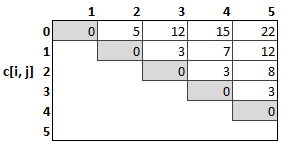
\includegraphics[width=0.45\textwidth]{q6-15-p1.png}
\captionof{figure}{Matriz $c$ preenchida após todas as iterações}
\label{fig:6.15-1}
\end{center}

O algorimto \proc{Analog-Cutting-Machinery} calcula o custo mínimo de corte da tora, com base na recorrência dada por $c[i, j]$.

\begin{codebox}
\Procname{$\proc{Analog-Cutting-Machinery}(p, l)$}
\li $\proc{Insert}(p, 0, 0)$
\li $\proc{Insert}(p, \attrib{p}{length}, l)$
\li $n \gets \attrib{p}{length}$
\li \For $i \gets 0$ \To $n-1$
\li \Do
        $c[i, i+1] \gets 0$
    \End
\li \For $k \gets 1$ \To $n$
\li \Do
        \For $i \gets 0$ \To $n - k - 1$
\li     \Do
            $j \gets i + k + 1$
\li         $c[i, j] \gets \infty$
\li         \For $m \gets i+1$ \To $j$
\li         \Do
                $aux \gets c[i, m] + c[m, j]$
\li             \If $aux < c[i, j]$
\li             \Then
                    $c[i, j] \gets aux$
                \End
            \End
\li         $c[i, j] = c[i, j] + p[j] - p[i]$
        \End 
    \End
\li \Return $c[0, n]$
\end{codebox}

O custo mínimo do corte da tora é retornado na posição $c[0, n]$. A tabela \ref{tbl:6-15-1} mostra o tempo de execução do algoritmo $\proc{Analog-Cutting-Machinery}$. Como as inserções em $p$ nas linhas 1-2 podem ser feitas em tempo $\Theta(n)$, o consumo total é $\Theta(n^3)$. já que as linhas 6-14 têm 3 \textit{loops} encadeados que tomam, no máximo, $n$ iterações cada um.

\begin{table}[H]
\centering
\begin{tabular}{|l|l|}
\hline
Linha                   & Tempo \\ \hline
1-2 & $\Theta(n)$ \\ \hline
3 & $\Theta(1)$ \\ \hline
4-5 & $\Theta(n)$ \\ \hline
6-14 & $\Theta(n^3)$ \\ \hline
15 & $\Theta(1)$ \\ \hline
Total & $\Theta(3n) + \Theta(n^3) = \Theta(n^3)$ \\ \hline
\end{tabular}
\caption{Tempo de execução}
\label{tbl:6-15-1}
\end{table}

\noindent \textbf{16. UVA 10066} (Torres gêmeas) Havia em um império antigo duas torres de formatos diferentes, situadas cada uma em uma cidade diferente. As torres eram construídas de lajotas circulares postas uma sobre a outra. Cada uma das lajotas era da mesma altura e tinha um raio inteiro. Não era de se espantar no entanto, que apesar de terem formatos diferentes, as duas torres tinham muitas lajotas em comum.

Mais de mil anos depois que elas foram construídas, o imperador ordenou que seus arquitetos removessem algumas das lajotas das duas torres de maneira que elas ficassem com a mesma forma e tamanho, e que ao mesmo tempo ficassem tão altas quanto possível. A ordem das lajotas nas novas
torres deveria ser a mesma que nas torres originais. O imperador achou que, desta maneira, as torres seriam capazes de permanecer como símbolo da harmonia e igualdade entre as duas cidades. Ele decidiu chamá-las então de torres gêmeas.

Agora, cerca de dois mil anos depois, desafiamos você a resolver um problema mais simples: dada a descrição das duas torres distintas, você deve encontrar o número de lajotas que haveria no mais alto par de torres gêmeas que pode ser construído delas.\\[6pt]


\noindent \textbf{17. PC 111106} (Carregamento de balsa) Balsas são usadas para transportar carros para a outra margem de um rio ou outro trecho de água. Considere balsas que sejam largas o suficiente para acomodar duas faixas de carros em todo o seu comprimento. Os carros entram nas faixas por um lado da balsa e saem, na outra margem, do outro lado da balsa.

A fila de carros para entrar na balsa é uma fila única e o operador direciona cada carro para uma das duas faixas da balsa - a faixa esquerda ou a faixa direita - de modo a balancear as duas faixas da balsa. Cada carro na fila tem um comprimento diferente, que é estimado pelo operador enquanto os carros estão na fila. Baseando-se nessas estimativas, o operador decide em qual das duas faixas cada carro deve embarcar, e embarca tantos carros da fila quanto possível. Escreva um programa que informe o operador para qual faixa ele deve direcionar cada carro de modo a maximizar o número de carros embarcados na balsa.\\[6pt]

\noindent \textbf{18. Problema 15-7 do CLRS} (Programando para maximizar o lucro) Suponha que você tem uma máquina e um conjunto de $n$ trabalhos, identificados pelos números $1, 2, \ldots, n$, para processar nessa máquina. Cada trabalho $j$ tem um tempo de processamento $t_j$ , um lucro $p_j$ e um prazo final $d_j$ . A máquina só pode processar um trabalho de cada vez, e o trabalho $j$ deve ser executado ininterruptamente por $t_j$ unidades de tempo consecutivas. Se o trabalho $j$ for concluído em seu prazo $d_j$ , você recebe um lucro $p_j$, mas, se ele for completado depois do seu prazo final, você não recebe nenhum lucro. Escreva um algoritmo para encontrar a ordem de execução dos trabalho que maximiza a soma dos lucros, supondo que todos os tempos de processamento são inteiros entre 1 e $n$. Qual é o tempo de execução do seu algoritmo?\\[6pt]
\textbf{Resposta:} Temos $a_1, a_2, a_3, \ldots, a_n$ trabalhos e cada trabalho $a_j$ tem um tempo de processamento $t_j$, lucro $p_j$ e prazo $d_j$.

Devemos ordenar os $a_n$ trabalhos de acordo com o prazo de entrega e, desta forma, podemos pensar na solução como uma variação do problema da mochila onde a \textbf{subestrutura ótima} é: se o lucro dos trabalhos $a[1..i]$ é máximo, então, o lucro de $a[1..i-1]$ também é máximo, desde que o prazo de entrega $d_i$ e $d_{i-1}$, respectivamente, seja respeitado.

Assim como no problema da mochila nós temos uma capacidade máxima $W$, aqui, temos um prazo máximo $D = d_n$ para executar o trabalho $a_n$, já que ordenamos os trabalhos pelo prazo de entrega.

Vamos definir por $w[i, j]$ o lucro máximo obtido processando os trabalhos $a_1, a_2, a_3, \ldots a_i$ no prazo de entrega $j$. A recorrência pode, então, ser definida da seguinte maneira:
\begin{equation*}
    w[i, j] =
    \begin{cases}
        0 & \text{, se } i = 0 \text{ ou } j = 0 \\
        w[i-1, j] & \text{, se } t_i > j \\
        \max \{w[i-1, j], w[i-1, j-t_i] + p_i\} & \text{, se } t_i \leq j
    \end{cases}
\end{equation*}

Note que o caso base é quando não executamos nenhum trabalho ou o prazo para processamento é nulo. O segundo caso se dá quando o tempo de processamento $t_i$ do trabalho $a_i$ é maior que o limite de prazo $j$. Percebemos, também, que a matriz $w[i, j]$ tem dimensões $n$x$D$ e será preenchida da esquerda para direita, de cima para baixo.

O algoritmo está implementado em \textit{maximum\_profit.py} e tem ordem de complexidade $\Theta(nD)$ já que a ordenação pode ser feita em tempo $\Theta(nlgn)$. Assim como o problema da mochila, $D$ representa o prazo máximo que temos para executar os trabalhos, o que corresponde a $d_n$ assim que o vetor $d$ é ordenado, o que faz com que o algoritmo seja pseudo-polinomial já que D não é, garantidamente, polinomial no tamanho da entrada.

Se considerarmos, $D = 1.000.000.000.000$, precisamos de 40 bits para representar este número, então, o tamanho da entrada é 40, mas o tempo de execução, neste caso, usa este fator de $D$, o que nos dá $O(2^{40})$.

Logo, o tempo de execução seria, de forma mais precisa, $O(n2^n)$, se a quantidade de bits para representar $D = n$, o que tornaria o algoritmo exponencial.\\[12pt]

\noindent 21. (Bandeiras) No dia da Bandeira na Rússia o proprietário de uma loja decidiu decorar a vitrine de sua loja com faixas de tecido das cores branca, azul e vermelha. Ele deseja satisfazer as seguintes condições: faixas da mesma cor não podem ser colocadas uma ao lado da outra. Uma faixa azul sempre está entre uma branca e uma vermelha, ou uma vermelha e uma branca. Escreva um programa que, dado o número n de faixas a serem colocadas na vitrine, calcule o número de maneiras de satisfazer as condições do proprietário.

\textbf{Exemplo:} Para $n = 3$, o resultado são as seguintes combinações: BVB, VBV, BAV, VAB.\\[6pt]
\textbf{Resposta:} Podemos pensar no processo de formação da combinação das cores da seguinte maneira: a primeira posição, obrigatoriamente, deve conter um B ou um V. Vamos fazer uma simulação iniciando com B que, ao final, basta multiplicarmos por 2 para termos o número total de combinações. No segundo nível teremos então duas possibilidades: V e A.

Percebemos então que, a cada vez que temos um A, temos apenas uma possibilidade no nível seguinte. Quando temos um B ou um V, temos duas novas possibilidades. Devemos ter o cuidado ao finalizar as combinações para que não haja nós adjacentes com o mesmo valor e, também, nenhuma terminação em A.

% Set the overall layout of the tree
\tikzstyle{level 1}=[level distance=1.5cm, sibling distance=5cm]
\tikzstyle{level 2}=[level distance=1.5cm, sibling distance=3cm]
\tikzstyle{level 3}=[level distance=1.5cm, sibling distance=2cm]
\tikzstyle{level 4}=[level distance=1.5cm, sibling distance=1cm]
\tikzstyle{level 5}=[level distance=1.5cm, sibling distance=0.5cm]

% Define styles for bags and leafs
\tikzstyle{bag} = [shape=ellipse, draw, align=center,
                   top color=white, bottom color=gray!20]
\tikzstyle{end} = [shape=rectangle, rounded corners, draw, align=center, fill=gray!40]

\begin{figure}[!h]
\centering
\begin{tikzpicture}[grow=right]
\node[bag] {$B$}
    child {
        node[bag] {$A$}
            child {
                node[bag] {$V$}
                    child {
                        node[bag] {$A$}
                        child {
                            node[bag] {$B$}
                                child {
                                    node[bag] {$V$}
                                    edge from parent 
                                    node[above] {}
                    			}
            			}
        			}
                    child {
                        node[bag] {$B$}
                            child {
                                node[bag] {$A$}
                                    child {
                                        node[bag] {$V$}
                                        edge from parent 
                                        node[above] {}
                        			}
                			}
                            child {
                                node[bag] {$V$}
                                    child {
                                        node[bag] {$B$}
                                        edge from parent 
                                        node[above] {}
                        			}
                			}
        			}
			}
    }
    child {
        node[bag] {$V$}
            child {
                node[bag] {$A$}
                    child {
                        node[bag] {$B$}
                            child {
                                node[bag] {$A$}
                                    child {
                                        node[bag] {$V$}
                                        edge from parent 
                                        node[above] {}
                        			}
                			}
                            child {
                                node[bag] {$V$}
                                    child {
                                        node[bag] {$B$}
                                        edge from parent 
                                        node[above] {}
                        			}
                			}
        			}
			}
            child {
                node[bag] {$B$}
                    child {
                        node[bag] {$A$}
                            child {
                                node[bag] {$V$}
                                    child {
                                        node[bag] {$B$}
                                        edge from parent 
                                        node[above] {}
                        			}
                			}
        			}
                    child {
                        node[bag] {$V$}
                            child {
                                node[bag] {$A$}
                                    child {
                                        node[bag] {$B$}
                                        edge from parent 
                                        node[above] {}
                        			}
                			}
                            child {
                                node[bag] {$B$}
                                    child {
                                        node[bag] {$V$}
                                        edge from parent 
                                        node[above] {}
                        			}
                			}
        			}
			}
    };
\end{tikzpicture}
\captionof{figure}{Árvore de combinações possíveis para $n = 6$}
\label{fig:6.21-1}
\end{figure}

Logo, percebemos que o número de combinações de $1..n-1$ cresce conforme a série de Fibonacci e, portanto, podemos calcular o número de maneiras de satisfazer as condições do proprietário com a própria recorrência que calcula a série de Fibonacci:
\begin{align*}
t(n) = \left\{\begin{array}{rl}
                    0, &\mbox{se $n = 0$} \\
                    1, &\mbox{se $n = 1$} \\
                    t(n - 1) + t(n - 2) + 1, &\mbox{se $n \geq 2$}
                \end{array} \right.
\end{align*}

Como temos duas possibilidades (iniciando a série com B ou V), basta multiplicarmos o resultado da série de Fibonacci(n) por 2 e teremos, então, o número de diferentes maneiras que podemos organizar as faixas de tecido na vitrine. O algoritmo \proc{Arrange-Flags} mostra a solução que, na verdade, é uma pequena alteração do algoritmo original de Fibonacci para programação dinâmica.

\begin{codebox}
\Procname{$\proc{Arrange-Flags}(n)$}
\li $f[0] \gets 0$
\li $f[1] \gets 1$
\li \For $i \gets 2$ \To $n$
\li \Do
        $f[i] \gets f[i-1] + f[i-2]$
    \End
\li \Return 2 * f[n]
\end{codebox}

Sendo assim, no exemplo supra citado, para $n = 6$, temos que o número de combinações possíveis é 16.

Obviamente o consumo de espaço e tempo do algoritmo é $\Theta(n)$, assim como é o original.

\noindent \textbf{3. mac338-2008, p2} Dado $n$ e uma cadeia de $n$ caracteres $s[1..n]$ que você acredita ser um texto corrompido, em que toda a pontuação foi removida (de modo que pareça com alguma coisa assim... "eraumavezumgatoxadrez..."). Você deseja reconstruir o documento, usando um dicionário, que está disponível na forma de uma função booleana $dict(.)$ para cada cadeia de caracteres w,

\begin{equation*}
    dict(.) =
    \begin{cases}
        true & \text{se $w$ é uma palavra válida} \\
        false & \text{caso contrário}
    \end{cases}
\end{equation*}

Escreva um algoritmo de programação dinâmica que, dado $n$ e uma cadeia de caracteres $s[1..n]$, determina se $s$ pode ser reconstituída como uma sequência de palavras válidas. O seu algoritmo deve consumir tempo $O(n^2)$. Justifique porque ele funciona (por exemplo explicando a validade da recorrência de onde ele foi derivado) e porque o seu consumo de tempo é $O(n^2)$.\\[12pt]

\noindent \textbf{3. mac338-2011, p2} Você conhece a tartaruga Yertle?

O trono de Yertle é composto de uma pilha de tartarugas, conforme a figura \ref{fig:6.23-1}.

\begin{center}
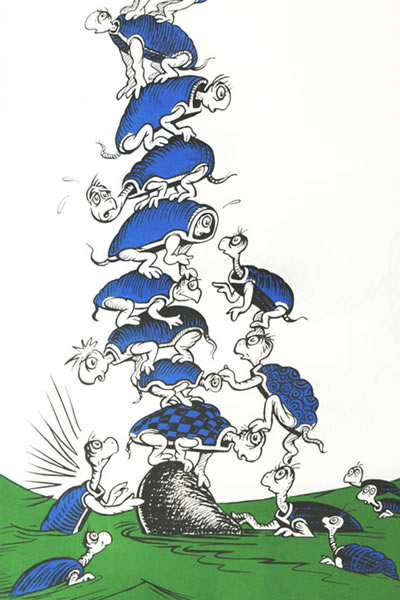
\includegraphics[width=0.45\textwidth]{q6-23}
\label{fig:6.23-1}
\end{center}

Cada tartaruga, ao se alistar para fazer parte do trono, fornece o seu peso e a sua força. A sua missão é determinar uma pilha de tartarugas, dentre as alistadas, o maior possível, em que nenhuma tartaruga quebre por entrar na pilha. O peso de cada tartaruga é dado em gramas, e a sua força é em gramas também.

A força de uma tartaruga indica quanto peso, incluindo o seu, ela aguenta. Ou seja, uma tartaruga de peso 300 gramas que tem força de 1000 gramas pode carregar 700 gramas de tartarugas sobre ela. Numa pilha válida de tartarugas, cada tartaruga tem força para sustentar as tartarugas que estão acima dela na pilha. Considere as três possíveis maneiras de ordenarmos as tartarugas:\\[6pt]

\noindent (i) em ordem decrescente de peso;\\[2pt]
(ii) em ordem decrescente de força;\\[2pt]
(iii) em ordem decrescente de força menos peso.\\[6pt]

\noindent (a) Para cada uma destas três ordens, prove ou dê um contra-exemplo para a seguinte afirmação: qualquer pilha válida de tartarugas pode ser reorganizada para que as tartarugas apareçam nesta ordem, de baixo para cima, e a pilha continue válida. Dica: a afirmação é verdadeira para apenas uma das ordens.\\[2pt]
\noindent (b) Seja n o número de tartarugas, $p[1..n]$ o peso das $n$ tartarugas e $f[1..n]$ a força das $n$ tartarugas.

Suponha que as tartarugas estão ordenadas na ordem correta (a que funciona das três acima) e que todas tem peso maior que zero. Seja $c[i, w]$ o número de tartarugas na maior pilha válida de tartarugas composta de tartarugas de 1 a $i$ com peso igual a $w$. (Se não houver pilha válida, deixe $c[i,w] = -1$.)

Escreva uma recorrência válida para $c[i, x]$ (acho que é w aqui). Não esqueça de definir o caso base da recorrência! Explique porque sua recorrência está correta, ou seja, prove (indutivamente) que $c[i,w]$ é o número de tartarugas na maior pilha válida de tartarugas composta de tartarugas de 1 a $i$ com peso igual a $w$.\\[2pt]
\noindent (c) A partir da sua recorrência, escreva (em pseudo-código, como nas aulas) um algoritmo de programação
dinâmica que, dados $n$, $p$ e $f$, representando os dados de $n$ tartarugas, determine e devolva o número de tartarugas em uma pilha válida máxima formada com estas tartarugas. O seu algoritmo deve claramente corresponder à sua recorrência.\\[2pt]
\noindent (d) Analise o consumo de tempo do seu algoritmo em função de $n$.
\clearpage
\end{comment}

\begin{center}
\textbf{\large{Lista 7}}
\end{center}

\noindent \textbf{1. (CRLS 22.2-1)} Simule o funcionamento da BFS no grafo da Figura 22.2(a) do CLRS (segunda edição) a partir do vértice 3, determinando os valores de $d$ e $\pi$ para cada vértice.

\textbf{Resposta:} Inicializamos os atributos $color$, $d$ e $\pi$ de cada vértice $v \in V$ do grafo com \const{white}, $\infty$ e \const{nil}, respectivamente, conforme a primeira iteração do algoritmo \proc{BFS}, exceto para o nó 3 que é o parâmetro $s$ neste caso, cujo $d = 0$ e sua cor é \const{gray}, conforme pode ser visto em \textbf{a)}.

Colocamos $s$ na fila e, então, visitamos a lista de adjacências de cada vértice a partir de $s$, sendo que $u$ é o vértice retirado da pilha - aquele cuja cor é \const{black} ao final do $for$ da linha 12.

Note que o valor de $d$ está dentro de cada vértice do grafo e, a cada novo vértice que descobrimos a partir de $u$, ou seja, aquele que ainda tem a cor \const{white}, marcamos em seu atributo $\pi$ o seu antecessessor - o próprio $u$ - que destacamos em laranja.

Note, também, que há casos em que nenhum novo vértice é descoberto, como em \textbf{d)}, por exemplo.

Quando a pilha estiver vazia, concluímos a execução do algoritmo. Note que, neste caso, o vértice 1 não pode ser atingido a partir de 3 e, portanto, seu antecessor $\pi$ fica marcado como \const{nil}. O vértice $s$ também tem seu antecessor \const{nil}, já que é a entrada da busca no grafo e isso ocorre sempre.

As arestas que estão destacadas formam a \textit{breadth-first tree} e o antecessor de cada nó da árvore é dado pelo atributo $\pi$ de cada vértice.

\begin{center}
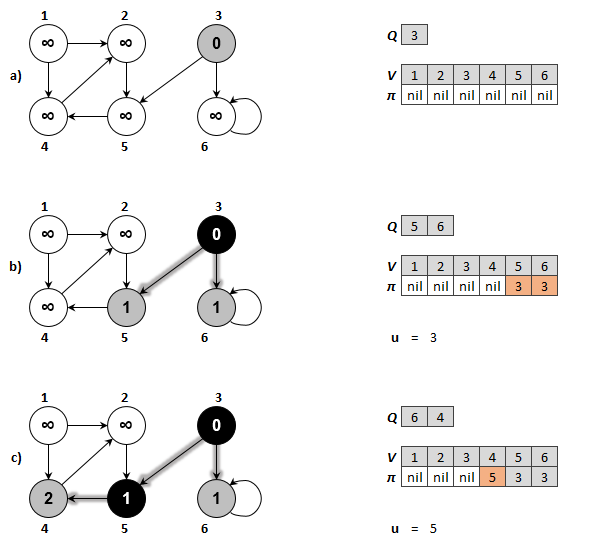
\includegraphics[width=0.8\textwidth]{q7-01-p1.png}
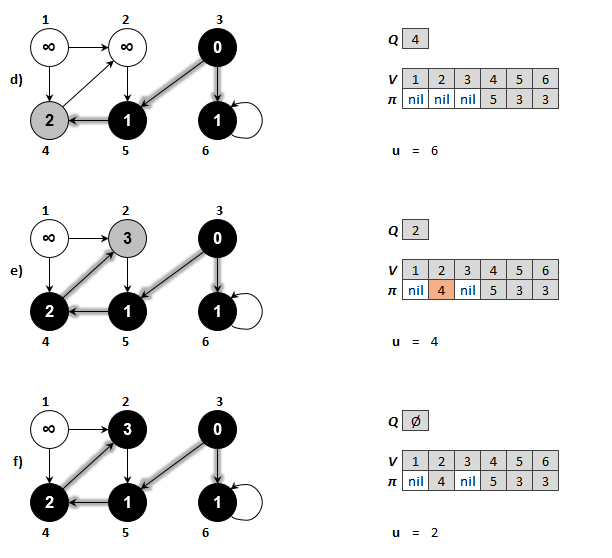
\includegraphics[width=0.8\textwidth]{q7-01-p2.png}
\captionof{figure}{Sequência das operações do algoritmo \proc{BFS}, sendo $s = 3$.}
\label{fig:7.1-1}
\end{center}

\noindent\textbf{2. (CRLS Ex. 22.2-2)} Simule o funcionamento da \proc{BFS} no grafo da Figura 22.3 do CLRS (segunda
edição) a partir do vértice $u$, determinando os valores de $d$ e $\pi$ para cada vértice.

\textbf{Resposta:} A mesma analogia aplicada na questão anterior pode ser utilizada aqui, mesmo tratando-se de um grafo não orientado, o algoritmo \proc{BFS} funciona em ambos os casos, conforme vimos em sala/CLRS.

\begin{center}
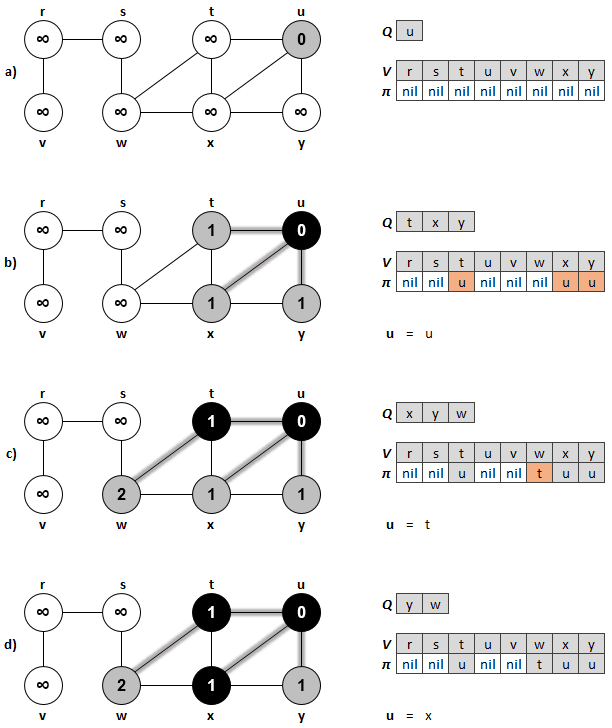
\includegraphics[width=0.8\textwidth]{q7-02-p1.png}
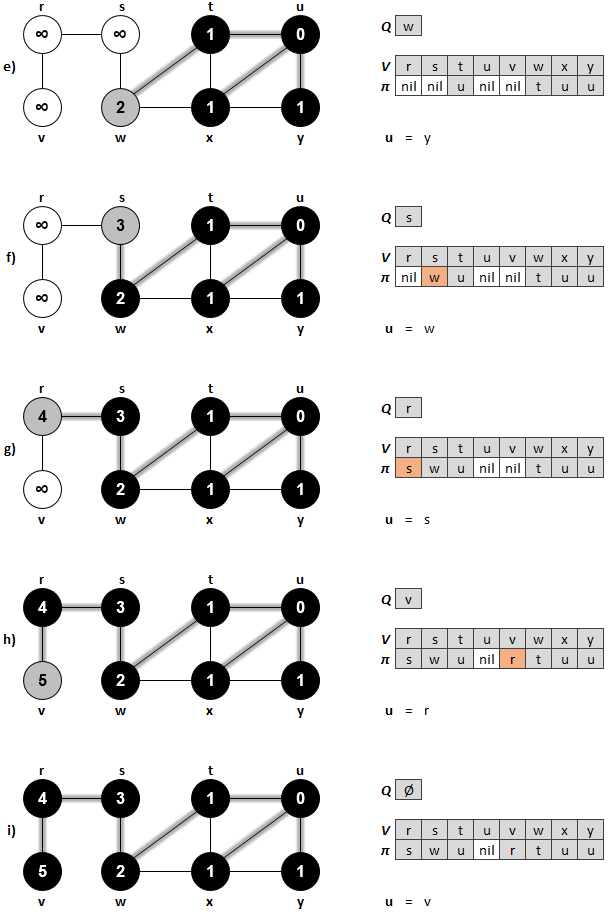
\includegraphics[width=0.8\textwidth]{q7-02-p2.png}
\captionof{figure}{Sequência das operações do algoritmo \proc{BFS}, sendo $s = u$.}
\label{fig:7.2-1}
\end{center}


\noindent\textbf{3. (CRLS 22.2-4)} Argumente que o valor de $d[u]$ atribuído ao vértice $u$ na BFS é independente da ordem em que os vértices das listas de adjacências são dados. Por outro lado, mostre, usando o exemplo da Figura 22.3 do CLRS, que a árvore BFS depende da ordem dos vértices nas listas de adjacências.

\textbf{Resposta:} O atributo $d$ de cada vértice $v$ é calculado uma única vez na linha 15, sendo que este valor é incrementado a cada nível da árvore que algoritmo descobre a partir de $s$.

Se tomarmos, por exemplo, o vértice $u$ do exercício anterior, de qualquer forma que organizarmos a sua lista de adjacências ($\{t, x, y\}, \{x, y, t\}, \{y, t, x\}$), o atributo $d$ de cada um destes vértices sempre será 1, o que nos mostra que eles estão em um nível imediatamente abaixo de $u$ na árvore.

Por outro lado, a ordem da lista de adjacências influencia na árvore resultante após a aplicação do algoritmo. Usando o mesmo exemplo que citamos no caso anterior, se tomarmos a lista de adjacências de $u$ na ordem $\{x, y, t\}$, a sub-árvore do segundo nível terá, agora, o vértice $x$ como a raiz, e não mais $t$, como visto no exercício 2. Consequentemente, o atributo $\pi$ do vértice $w$ também muda, já que $x$, agora, passa a ser o seu antecessor.

\begin{center}
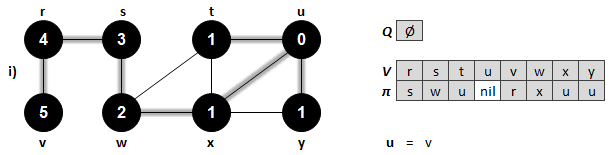
\includegraphics[width=0.8\textwidth]{q7-03.png}
\captionof{figure}{Árvore resultante do algoritmo \proc{BFS}, sendo $s = u$ e a lista de adjacências na ordem $\{x, y, t\}$.}
\label{fig:7.3-1}
\end{center}

\noindent\textbf{4. (CRLS 22.2-5)} Considere um grafo orientado $D = (N, A)$. Dê um exemplo de um conjunto $A_\pi \subseteq A$ de arcos em $D$ que formam uma árvore tal que, entre quaisquer dois nós $u$ e $v$ em $D$, o único caminho entre $u$ e $v$ em $A_\pi$ é um caminho mínimo em $D$ entre $u$ e $v$, porém, $A_\pi$ jamais seria produzida por uma execução da BFS em $D$, independente da ordem dos nós nas listas de adjacências de $D$ e do nó inicial $s$.

\textbf{Resposta:} Seja o conjunto de arcos $A_\pi$ destacados no grafo da figura \ref{fig:7.4-1}.
\begin{center}

\includegraphics[width=0.8\textwidth]{q7-04-p1.png}
\captionof{figure}{Grafo orientado $D = (N, A)$.}
\label{fig:7.4-1}
\end{center}

Note que, independente da ordem dos elementos adjacentes a $s$, $t$ e $u$, essa representação jamais poderá ser obtida pela \proc{BFS}. A ordem das listas de adjacências dos elementos $t$ e $u$ também não influenciam na forma com que a árvore será gerada. A figura \ref{fig:7.4-2} mostra o resultado da execução da \proc{BFS}, bem como a lista de adjacências em ordens diferentes em cada caso.
\begin{center}
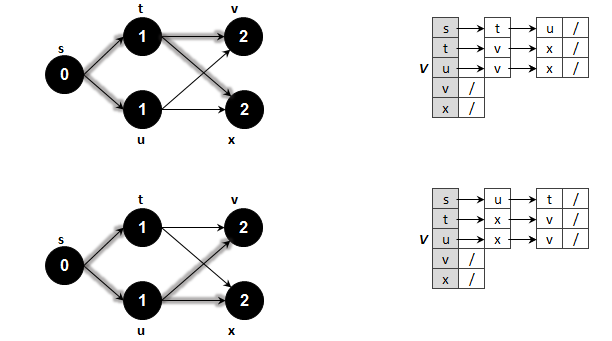
\includegraphics[width=0.8\textwidth]{q7-04-p2.png}
\captionof{figure}{Execução da \proc{BFS} no grafo orientado $D = (N, A)$ com a lista de adjacências em duas ordens distintas.}
\label{fig:7.4-2}
\end{center}


\noindent\textbf{5.} Escreva uma versão não recursiva da busca em profundidade.

\textbf{Resposta:} Podemos utilizar uma pilha como apoio para aprofundar na lista de adjacências de cada nó da árvore, substituindo a recursão.

Além disso, nós usamos uma fila FIFO para a lista de adjacências de cada vértice $u$ e, assim que um novo vértice $v$ adjacente à $u$ é encontrado e ele ainda não foi visitado, nós o visitamos e empilhamos $v$ em $S$.

Note que nós somente retiramos $u$ da pilha (linha 11 da \proc{DFS-Visit}) quando todos os vértices da lista de adjacências dele foram visitados, ou seja, o momento em que devemos marcar $u$ como finalizado (sub-rotina \proc{Blacken}).

Outro ponto importante é que, como visto na linha 12 da \proc{Iterative-DFS}, o vértice $s$ que dá origem à busca tem seu ancestral como $nil$, o que garante o funcionamento da mesma forma que a \proc{Dfs} original. Isso também garante que a busca funciona nos casos em que tivermos mais de uma componente conexa no grafo.

\textbf{Consumo de tempo:} O \textit{loop} das linhas 2-8 da \proc{Iterative-DFS} tomam $\Theta(V)$ para inicializar cada vértice $u \in V[G]$ + $\Theta(E)$ para montar a fila de adjacências de cada vértice $u$. As sub-rotinas \proc{Blacken}, \proc{Grayen}, bem como as operações na fila/pilha tomamm $\Theta(1)$. O \textit{loop} das linhas 10-13 consome tempo $\Theta(V)$, ou seja, executa no máximo uma vez para cada vértice $v \in G$, já que \proc{DFS-Visit} é executado apenas em vértices que ainda não foram descobertos - àqueles que ainda são brancos. Como a fila de adjacências é visitada no máximo uma vez na sub-rotina \proc{DFS-Visit} e a soma do comprimento da fila de adjacências de cada vértice $v$ é $\Theta(E)$, o tempo gasto na \proc{DFS-Visit} é $O(E)$.

Portanto, o consumo de tempo total será $O(V + E)$, o que mantém o comportamento assintótico original da \proc{DFS}.

\begin{codebox}
\Procname{$\proc{Iterative-DFS}(G)$}
\li \Comment let $S$ be an empty stack
\li \For each vertex $u \in V[G]$
\li \Do
        $\id{color}[u] \gets \const{white}$
\li     $\id{\pi}[u] \gets \const{nil}$
\li     $n \gets \id{Adj}[u].length$
\li     \For $i \gets n$ to $1$
\li     \Do
            $v \gets \id{Adj}[u][i]$
\li         $\proc{Enqueue}(\id{Qadj}[u], v)$
        \End
    \End
\li $time \gets 0$
\li \For each vertex $u \in V[G]$
\li \Do
        \If $\id{color}[u] == \const{white}$
\li     \Then 
            $\proc{Grayen}(u, \const{nil})$
\li         $\proc{DFS-Visit}(u)$
    \End
\end{codebox}

\begin{codebox}
\Procname{$\proc{DFS-Visit}(s)$}
\li $\proc{Push}(S, s)$
\li \While $S \neq \emptyset$
\li \Do
        $u \gets \proc{Top}(S)$
\li     \If $\id{Qadj}[u] \neq \emptyset$
\li     \Then
            $v \gets \proc{Dequeue}(\id{Qadj}[u])$
\li         \If $\id{color}[v] == \const{white}$
\li         \Then
                $\proc{Grayen}(v, u)$
\li             $\proc{Push}(S, v)$
\li         \End
        \Else
\li         $\proc{Blacken}(u)$
\li         $\proc{Pop}(S)$
        \End
    \End
\end{codebox}

\begin{codebox}
\Procname{$\proc{Grayen}(v, u)$}
\li $\id{color}[v] \gets \const{gray}$
\li $time \gets time + 1$
\li $\id{d}[v] \gets time$
\li $\id{\pi}[v] \gets u$
\end{codebox}

\begin{codebox}
\Procname{$\proc{Blacken}(u)$}
\li $\id{color}[u] \gets \const{black}$
\li $time \gets time + 1$
\li $\id{f}[u] \gets time$
\end{codebox}


\noindent\textbf{6.} Execute uma busca em profundidade a partir do vértice 0 no grafo orientado dado pelas listas de adjacência a seguir. Exiba o rastreamento da busca.\\[6pt]
\noindent0: 1 4\\
1: 2 5\\
2: 3\\
3: 7\\
4: 8\\
5: 4\\
6: 5 10 2\\
7: 11 6\\
8: 9\\
9: 5 8\\
10: 9\\
11: 10\\

\textbf{Resposta:} A figura \ref{fig:7.6-1} mostra o grafo formado pela lista de adjacências dada, bem como o rastreamento no momento em que o vértice 3, 6 e 8 são descobertos, e o resultado final da \proc{DFS} ao final de todas as chamadas recursivas, respectivamente. Os tempos $d$ e $f$ estão no vetor à direita e, também, acima de cada vértice.

\begin{center}
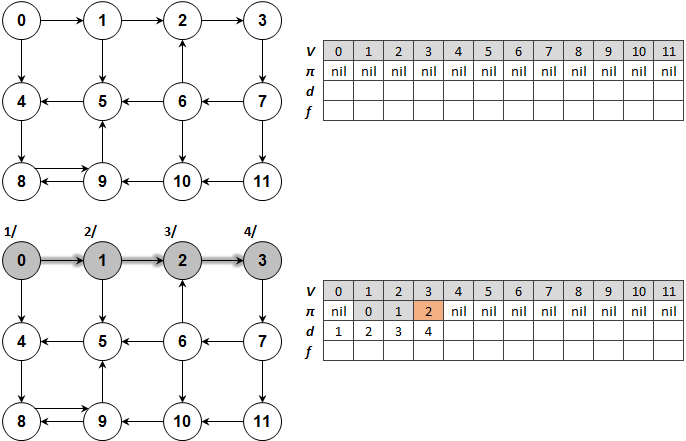
\includegraphics[width=0.9\textwidth]{q7-06-p1.png}
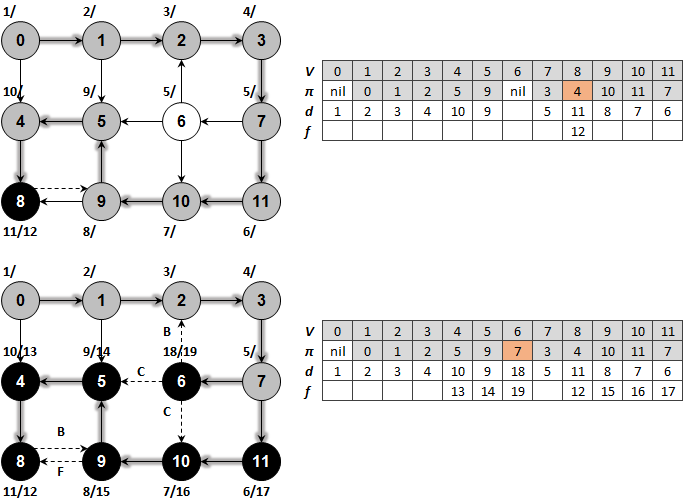
\includegraphics[width=0.9\textwidth]{q7-06-p2.png}
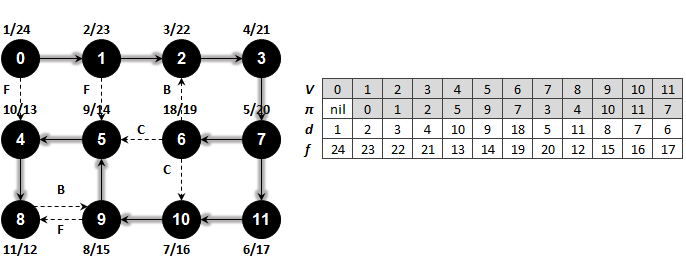
\includegraphics[width=0.9\textwidth]{q7-06-p3.png}
\captionof{figure}{Rastreamento da \proc{DFS} na lista de adjacências dada.}
\label{fig:7.6-1}
\end{center}


\noindent\textbf{7. (CRLS 22.3-1)} Desenhe uma tabela $3 x 3$, com as linhas e colunas indexadas pelas cores branco, cinza e preto. Em cada entrada $(i, j)$, indique se, em qualquer ponto durante uma \proc{DFS} de um grafo orientado, pode existir um arco de um nó de cor $i$ para um nó de cor $j$. Para cada arco possível, indique as classificações que ele pode ter (de árvore, de retorno, para frente, cruzado). Faça um segundo quadro considerando um grafo não orientado.\\[6pt]
As tabelas \ref{tbl:7-7-1} e \ref{tbl:7-7-2} mostram as classificações dos arcos para o grafo orientado e não orientado, respectivamente.

As siglas significam \textit{\textbf{T}ree}, \textit{\textbf{B}ack}, \textit{\textbf{C}ross} e \textit{\textbf{F}orward edge}.

\begin{table}[H]
\centering
\begin{tabular}{l | lll}
\textbf{}      & \textbf{White} & \textbf{Gray} & \textbf{Black} \\
\hline
\textbf{White} & x              & x             & x              \\
\textbf{Gray}  & T              & B             & F/C            \\
\textbf{Black} & x              & x             & B           
\end{tabular}
\caption{Classificação dos arcos no grafo orientado para a \proc{DFS}.}
\label{tbl:7-7-1}
\end{table}

\begin{table}[H]
\centering
\begin{tabular}{l | lll}
\textbf{}      & \textbf{White} & \textbf{Gray} & \textbf{Black} \\
\hline
\textbf{White} & x              & x             & x              \\
\textbf{Gray}  & T              & B             & x              \\
\textbf{Black} & x              & B             & B               
\end{tabular}
\caption{Classificação dos arcos no grafo não orientado para a \proc{DFS}.}
\label{tbl:7-7-2}
\end{table}

\noindent\textbf{8. (CRLS 22.3-2)} Mostre como a \proc{DFS} funciona no grafo da Figura 22.6 do CLRS (segunda
edição). Assuma que o laço das linhas 5-7 da \proc{DFS} visitam os vértices em ordem alfabética, e que
os vértices se encontram em ordem alfabética nas listas de adjacências. Mostre os valores de $d$ e $f$
para cada vértice ao final da \proc{DFS}.

\textbf{Resposta:} A figura \ref{fig:7.8-1} mostra o rastreamento da \proc{DFS} em 3 momentos distintos: quando todos os vértices adjacentes à $w$ são visitados, todos os vértices adjacentes à $t$ são visitados e a árvore com todas as chamadas recursivas concluídas, respectivamente.

Os valores $d$ e $f$, bem como o antecessor de cada vértice dado por $\pi$ estão na tabela de rastreamento abaixo de cada imagem. Os tipos de arestas também estão devidamente destacados.

\begin{center}
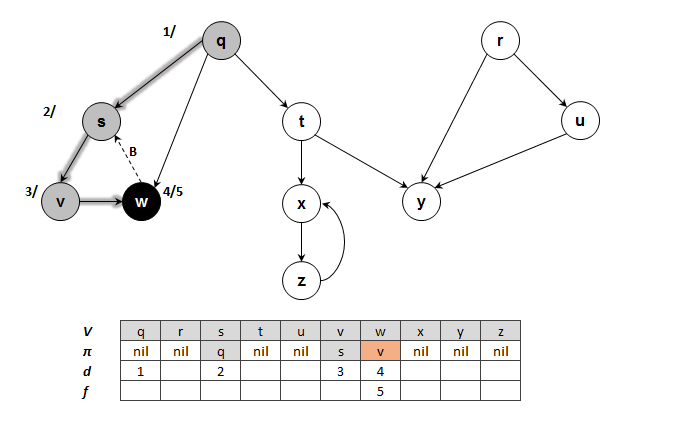
\includegraphics[width=0.9\textwidth]{q7-08-p1.png}
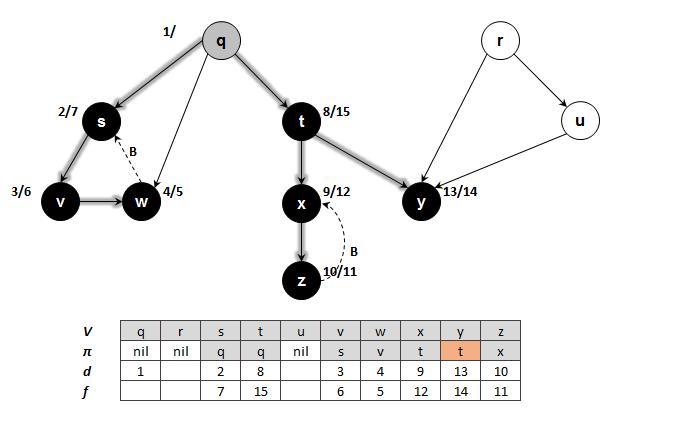
\includegraphics[width=0.9\textwidth]{q7-08-p2.png}
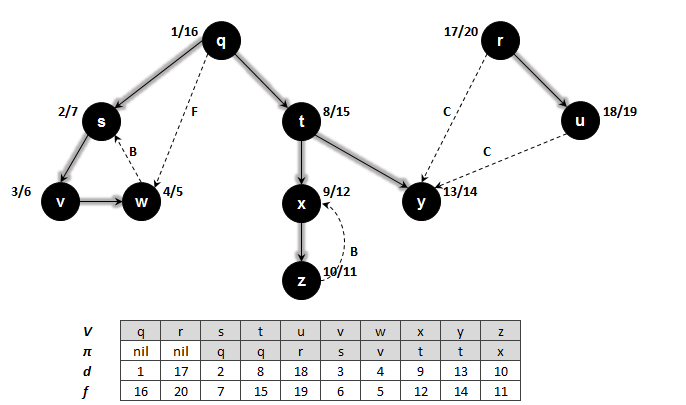
\includegraphics[width=0.9\textwidth]{q7-08-p3.png}
\captionof{figure}{Rastreamento da \proc{DFS} na figura 22.6 do CLRS.}
\label{fig:7.8-1}
\end{center}

\noindent\textbf{9. (CRLS 22.3-7)} Mostre um contraexemplo para a conjectura que se existe um caminho de $u$ a $v$ em um grafo orientado $G$, e se $d[u] < d[v]$ numa DFS de $G$, então $v$ é descendente de $u$ na floresta DFS produzida.

Podemos observar a própria árvore à esquerda da figura 22.5 (c) do CLRS como um contraexemplo. Seja a DFS produzida a partir de $s$, se tomarmos os vértices $x$ e $w$, $d[x] < d[w]$, existe um caminho de $x$ a $w$, mas $w$ não é descendente de $x$.
\begin{center}
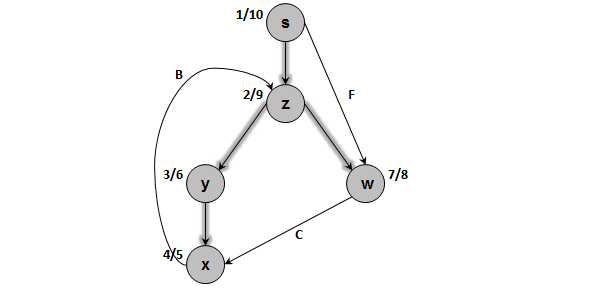
\includegraphics[width=0.8\textwidth]{q7-09.png}
\captionof{figure}{Contraexemplo utilizando parte do grafo da figura 22.5 (c) do CLRS.}
\label{fig:7.9-1}
\end{center}

\noindent\textbf{10. (CRLS 22.3-8)} Mostre um contraexemplo para a conjectura que se existe um caminho de $u$
a $v$ em um grafo orientado $G$, então qualquer \proc{DFS} deve resultar em $d[v] \leq f[u]$.

A figura \ref{fig:7.10-1} mostra um contraexemplo da conjectura. Temos um caminho de $u$ a $v$ no grafo, porém, aplicando a \proc{DFS} a partir de $s$, temos que $d[v] > f[u]$.
\begin{center}
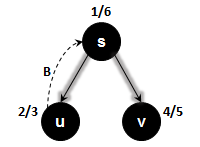
\includegraphics[width=0.28\textwidth]{q7-10.png}
\captionof{figure}{Contraexemplo da conjectura dada.}
\label{fig:7.10-1}
\end{center}


\noindent\textbf{11. (CRLS 22.3-10)} Mostre como um vértice $u$ num grafo orientado pode terminar sozinho numa árvore de uma floresta \proc{DFS} mesmo tendo arcos saindo e entrando dele em $G$.

A figura \ref{fig:7.11-1} mostra um exemplo onde o vértice $u$ pode ficar sozinho numa árvore de uma floresta \proc{DFS} gerada a partir do vértice $s$.
\begin{center}
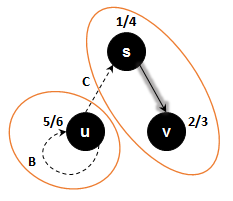
\includegraphics[width=0.33\textwidth]{q7-11-p1.png}
\captionof{figure}{Exemplo onde o vértice $u$ pode ficar isolado.}
\label{fig:7.11-1}
\end{center}


Um outro exemplo pode ser visto na figura \ref{fig:7.11-2}, sendo que cada árvore é formada por um único vértice, já que a busca começa em $v$.
\begin{center}
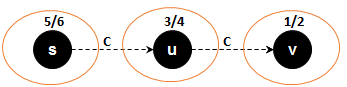
\includegraphics[width=0.48\textwidth]{q7-11-p2.png}
\captionof{figure}{Segundo exemplo onde o vértice $u$ pode ficar isolado.}
\label{fig:7.11-2}
\end{center}

\textbf{13.} Escreva uma generalização comum das buscas em largura e em profundidade. Sua função deve usar uma estrutura de dados auxiliar que pode operar como fila ou como pilha. Se a estrutura operar como fila, a função executa busca em largura, e se operar como pilha, a função executa busca em profundidade.\\[6pt]
\textbf{Resposta:} Basta efetuarmos algumas alterações na versão iterativa da \proc{Iteratve-DFS} para que a estrutura de dados opere de forma tal que ambas as buscas são atendidas. Basicamente, a ordem em que um vértice descoberto é incluído na pilha: se for busca em profundidade, incluímos no topo da pilha, se for em largura, incluímos na base (\proc{Push-Left}).

No caso de busca em largura, a sub-rotina \proc{Grayen} atualiza $d[v] = d[u] + 1$, considerando o caso onde o vértice é a origem da busca ($d[v] = 0$). Além disso, \proc{Blacken} só atualiza $f[u]$ se for uma busca em profundidade.

\textbf{Consumo de tempo:} As alterações não afetam o consumo de tempo obtido na \proc{Iterative-DFS}, permanecendo $O(V + E)$, o que mantém o comportamento original tanto da \proc{DFS}, quanto da \proc{BFS}.

\begin{codebox}
\Procname{$\proc{GFS}(G, type)$}
\li \Comment let $S$ be an empty stack
\li \For each vertex $u \in V[G]$
\li \Do
        $\id{color}[u] \gets \const{white}$
\li     $\id{\pi}[u] \gets \const{nil}$
\li     $n \gets \id{Adj}[u].length$
\li     \For $i \gets n$ to $1$
\li     \Do
            $v \gets \id{Adj}[u][i]$
\li         $\proc{Enqueue}(\id{Qadj}[u], v)$
        \End
    \End
\li $time \gets 0$
\li \For each vertex $u \in V[G]$
\li \Do
        \If $\id{color}[u] == \const{white}$
\li     \Then 
            $\proc{Grayen}(u, \const{nil})$
\li         $\proc{GFS-Visit}(u)$
    \End
\end{codebox}

\begin{codebox}
\Procname{$\proc{GFS-Visit}(s)$}
\li $\proc{Push}(S, s)$
\li \While $S \neq \emptyset$
\li \Do
        $u \gets \proc{Top}(S)$
\li     \If $\id{Qadj}[u] \neq \emptyset$
\li     \Then
            $v \gets \proc{Dequeue}(\id{Qadj}[u])$
\li         \If $\id{color}[v] == \const{white}$
\li         \Then
                $\proc{Grayen}(v, u)$
\li             \If $type == \const{bfs}$
\li             \Then
                    $\proc{Push-Left}(S, v)$
\li             \Else
\li                 $\proc{Push}(S, v)$
                \End
            \End
\li     \Else
\li         $\proc{Blacken}(u)$
\li         $\proc{Pop}(S)$
        \End
    \End
\end{codebox}

\begin{codebox}
\Procname{$\proc{Grayen}(v, u)$}
\li $\id{color}[v] \gets \const{gray}$
\li $\id{\pi}[v] \gets u$
\li \If $type == \const{bfs}$
\li \Then
        \If $u == \const{nil}$ \Comment it is a source vertex of a component
\li     \Then
            $\id{d}[v] \gets 0$
\li     \Else
\li         $\id{d}[v] \gets \id{d}[u] + 1$
        \End
\li \Else
\li     $time \gets time + 1$
\li     $\id{d}[v] \gets time$
    \End
\end{codebox}

\begin{codebox}
\Procname{$\proc{Blacken}(u)$}
\li $\id{color}[u] \gets \const{black}$
\li \If $type == \const{dfs}$
\li \Then
        $time \gets time + 1$
\li     $\id{f}[u] \gets time$
    \End
\end{codebox}

\noindent\textbf{14.} Escreva um algoritmo que decida se um grafo é conexo. Analise o seu consumo de tempo.\\[6pt]
\textbf{Resposta:} Um grafo é conexo se e somente se, para cada par $s$ e $t$ de seus vértices, existe um caminho com origem $s$ e término $t$.

Podemos fazer uma alteração no algoritmo da \proc{DFS} para contar o número de componentes conexas do grafo e executar a \proc{DFS} usando cada vértice $u \in V[G]$ como origem da busca. Se houver uma única componente conexa para a busca a cada execução, o grafo é conexo.

Assumindo que os vértices estão organizados em uma pilha, utilizamos as rotinas \proc{Pop} e \proc{Push-Left}, para remover um elemento da última posição da fila e inseri-lo na primeira posição, respectivamente, de modo que todos os vértices sejam origem da busca uma vez.

\textbf{Consumo de tempo:} A mudança em $\proc{Connected-DFS}$ não muda o comportamento assintótico original do algoritmo, que permanece $\Theta(V + E)$.

As operações na pilha gastam $\Theta(1)$ na rotina $\proc{Graph-Connected}$, bem como as demais instruções. Como nós fazemos a busca uma vez para cada vértice, temos que o consumo de tempo total será $\Theta(V(V + E))$.

\begin{codebox}
\Procname{$\proc{Graph-Connected}(G)$}
\li	$n \gets V[G].length$
\li \While $n > 1$
\li \Do
        $count = \proc{Connected-DFS}(G)$
\li     \If $count > 1$
\li     \Then 
            \Return \const{false}
        \End
\li     $u \gets \proc{Pop}(V[G])$
\li     $\proc{Push-Left}(V[G], u)$
\li     $n \gets n - 1$
    \End
\li \Return \const{true}
\end{codebox}

\begin{codebox}
\Procname{$\proc{Connected-DFS}(G)$}
\li \For each vertex $u \in V[G]$
\li \Do
        $\id{color}[u] \gets \const{white}$
\li     $\id{\pi}[u] \gets \const{nil}$
    \End
\li $time \gets 0$
\li $count \gets 0$
\li \For each vertex $u \in V[G]$
\li \Do
        \If $\id{color}[u] == \const{white}$
\li     \Then 
            $count \gets count + 1$
\li         $\proc{DFS-Visit}(u)$
        \End
    \End
\li \Return count
\end{codebox}

\noindent\textbf{15.} Escreva um algoritmo que determine o número de componentes conexas de um grafo. Analise o seu consumo de tempo.

\textbf{Resposta:} A rotina \proc{Connected-DFS} do exercício 7-14 já retorna a quantidade de componentes conexas de um grafo $G$.

O consumo de tempo é o mesmo da \proc{DFS} original, ou seja, $\Theta(V + E)$.\\[6pt]

\noindent\textbf{16.} Um grafo $G = (V, E)$ é bipartido se seu conjunto de vértices $V$ pode ser bipartido em dois conjuntos disjuntos de vértices $A$ e $B$ e toda aresta de $E$ tem uma ponta em $A$ e outra em $B$. Escreva um algoritmo que, dado um grafo, determine se o grafo é ou não bipartido. Analise o seu consumo de tempo.

\textbf{Resposta:} Podemos efetuar uma alteração na \proc{BFS}, de modo que quando um vértice $u$ encontra um vértice $v$ que já foi visitado, ou seja, já está \const{gray}, verificamos se a profundidade tanto de $u$ quanto de $v$ é par, ou se ambas são ímpar.

Isso implica que $d[u]$ e $d[v]$ têm a mesma paridade e, portanto, o grafo \textbf{não é bipartido}.

\textbf{Consumo de Tempo:} A modificação não altera o comportamento assintótico original da \proc{BFS} que permanece $O(V + E)$.

\begin{codebox}
\Procname{$\proc{BFS-Partite}(G, s)$}
\li \For each vertex $u \in V[G] - \{s\}$
\li \Do
        $u.\id{color} \gets \const{white}$
\li     $u.\id{d} \gets \infty$
\li     $u.\id{partition} \gets 0$
    \End
\li $s.\id{color} \gets \const{gray}$
\li $s.\id{d} \gets 0$
\li $s.\id{partition} \gets 1$
\li $Q \gets \emptyset$
\li $\proc{Enqueue}(Q, s)$
\li \While $Q \neq \emptyset$
\li \Do
        $u \gets \proc{Dequeue}(Q)$
\li     \For each $v \in G.\id{Adj}[u]$
\li     \Do
            \If $u.\id{partition} == v.\id{partition}$
\li         \Then
                \Return $\const{false}$
\li         \Else
\li             \If $v.\id{color} == \const{white}$
\li             \Then 
                    $v.\id{color} \gets \const{gray}$
\li                 $v.\id{d} \gets u.\id{d} + 1$
\li                 $v.\id{partition} \gets 3 - u.\id{partition}$
\li                 $\proc{Enqueue}(Q, v)$
                \End
            \End
        \End
\li     $u.\id{color} \gets \const{black}$
    \End
\li \Return $\const{true}$
\end{codebox}


\noindent\textbf{17. (CLRS 22.2-8)} Dada uma árvore $T = (V, E)$, o diâmetro de $T$ é o número $\max\{d(u, v) : u, v \in V \}$, onde $d(u, v)$ é a distância entre $u$ e $v$ em $T$. Escreva um algoritmo que, dado $T$, determine o diâmetro de $T$. Analise o seu consumo de tempo.

\textbf{Resposta:} Conforme enunciado, o diâmetro de uma árvore $T$ é a distância mais longa entre quaisquer dois nós $u$ e $v$ da árvore.

Para calcular o diâmetro podemos executar a \proc{BFS} usando cada vértice $v \in V$ como fonte da busca, retornando o maior valor de $d$ para cada busca. A maior distância será, então, o diâmetro de $T$.

A linha 19 deve retornar o número de vértices que tem o caminho mais longo de $u$ a $v$. Repare que somamos 1 devido à inicialização de $s.d = 0$.

\textbf{Consumo de Tempo:} A inclusão da linha 18 não muda o consumo de tempo da \proc{BFS}, que continua $O(V + E)$. Como executamos a \proc{BFS} uma vez para cada vértice no \textit{loop} da linha 3 da rotina $\proc{Tree-Diameter}$, temos que o tempo total será $O(V(V + E))$.

\begin{codebox}
\Procname{$\proc{Tree-Diameter}(T)$}
\li $diameter \gets 0$
\li \For each $u \in T$
\li \Do
        $max\_d = \proc{BFS}(T, u)$
\li     \If $max\_d > diameter$
\li     \Then 
            $diameter \gets max\_d$
        \End
    \End
\li \Return $diameter$
\end{codebox}

\begin{codebox}
\Procname{$\proc{BFS}(T, s)$}
\li \For each vertex $u \in V[T] - \{s\}$
\li \Do
        $u.\id{color} \gets \const{white}$
\li     $u.\id{d} \gets \infty$
\li     $u.\id{\pi} \gets \const{nil}$
    \End
\li $s.\id{color} \gets \const{gray}$
\li $s.\id{d} \gets 0$
\li $s.\id{\pi} \gets \const{nil}$
\li $Q \gets \emptyset$
\li $\proc{Enqueue}(Q, s)$
\li \While $Q \neq \emptyset$
\li \Do
        $u \gets \proc{Dequeue}(Q)$
\li     \For each $v \in T.\id{Adj}[u]$
\li     \Do
            \If $v.\id{color} == \const{white}$
\li         \Then 
                $v.\id{color} \gets \const{gray}$
\li             $v.\id{d} \gets u.\id{d} + 1$
\li             $v.\id{\pi} \gets u$
\li             $\proc{Enqueue}(Q, v)$
            \End
        \End
\li     $u.\id{color} \gets \const{black}$
    \End
\li \Return $u.\id{d} + 1$
\end{codebox}
\clearpage

\begin{center} 
\textbf{\large{Lista 8}}
\end{center}

\noindent\textbf{1. (CRLS 23.1-1)} Seja $e$ uma aresta de custo mínimo em um grafo $G$ com custos nas arestas. É verdade que $e$ pertence a alguma MST de $G$? É verdade que $e$ pertence a toda MST de $G$?\\[6pt]
\textbf{Resposta:} Seja $A$ um subconjunto de arestas de alguma MST $T$, tal que $(u, v) \notin A$. Para escolher uma aresta para ser adicionada em $A$, todas as arestas que atravessam um corte $(S, V - S)$ são consideradas. Como o corte deve respeitar $A$ e a aresta $(u, v)$ tem peso mínimo, ela será escolhida para ser incluída em $A$, o que dá origem a uma nova MST $T'$, onde $A \cup \{(u, v)\} \subseteq T'$.

\textbf{É verdade que $e$ pertence a toda MST de $G$?}
Não é verdade. Se tomarmos uma aresta $(u, v) \in E$ de uma MST $T$ que tenha custo mínimo $k$ e substituirmos por outra $(u, w)$ que não está em $T$ de custo $k = l$, teremos uma nova MST $T'$, ou seja, é o caso onde há empate na escolha da aresta segura para ser incluída na árvore. Portanto, $e$ não pertence a toda MST de $G$.

Na figura \ref{fig:8.1-1}, basta substituirmos a aresta $(b, c)$ pela $(b, d)$ e teremos uma nova MST de mesmo custo mínimo.
\begin{center}
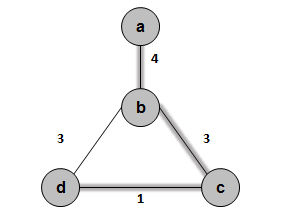
\includegraphics[width=0.4\textwidth]{q8-01.png}
\captionof{figure}{MST com mais de uma aresta de mesmo custo.}
\label{fig:8.1-1}
\end{center}

\noindent\textbf{2.} Suponha que os custos das arestas de um grafo conexo são distintos dois a dois (ou seja, não há duas arestas com o mesmo custo). Mostre que o grafo tem uma única MST.\\[6pt]
\textbf{Resposta:} Seja $m$ a quantidade de arestas em um grafo ponderado $G(V, E, w)$. Como não há arestas com pesos iguais, temos que os pesos são estritamente crescentes, ou seja, $w_1 < w_2 < w_3 < \ldots < w_m$.

\textbf{Prova por contradição:}\\
Vamos assumir que existem duas MST's $T$ e $T'$ no grafo. Seja $e_1$ uma aresta de menor custo que aparece em uma dessas MST's. Sem perda de generalidade, digamos que $e_1 \subseteq T$. Como $T'$ é uma MST, $T' \cup \{e_1\}$ contém um ciclo $C$ e, portanto, uma das arestas deste ciclo, digamos $e_2$, não está em $T$.

Note que $w(e_1) < w(e_2)$ e $T'' = T' \cup \{e_1\}$ \textbackslash $\{e_2\}$ é uma árvore geradora. O peso total de $T''$ é menor que o peso total de $T'$, mas isso é uma contradição, já que nós assumimos que $T'$ é uma MST. Em outras palavras, para que $T$ e $T'$ fossem MST's, deveríamos ter $w(e_1) = w(e_2)$, mas isso é impossível, já que os pesos são diferentes.

\begin{center}
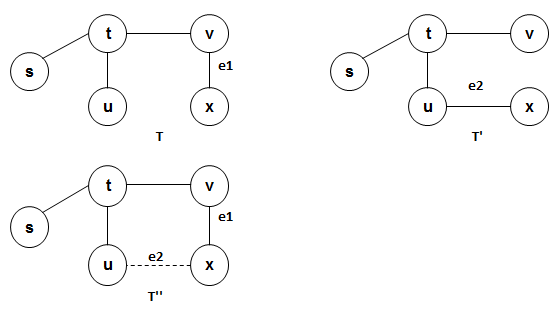
\includegraphics[width=0.8\textwidth]{q8-02.png}
\captionof{figure}{Exemplo de grafo com uma única MST com pesos nas arestas diferentes.}
\label{fig:8.2-1}
\end{center}

\noindent\textbf{3.} Suponha que os custos das arestas de um grafo conexo são distintos dois a dois. Seja $C$ um ciclo não trivial. É verdade que a aresta de custo mínimo em $C$ pertence à (única) MST do grafo?\\[6pt]
\textbf{Resposta:} Sim, é verdade. Seja $e$ a aresta de custo mínimo em $C$. Se $e$ não estivesse na única MST do grafo, ao removermos qualquer outra aresta do ciclo $C$ de custo maior para incluir $e$, teríamos uma MST de custo menor.\\[6pt]

\noindent\textbf{4. (CRLS 23.1-2)} Prove ou desprove a seguinte afirmação: Dado um grafo $G$ com pesos nas arestas, um conjunto de arestas $A$ de $G$, e um corte que respeita $A$, toda aresta que cruza o corte e que é segura para $A$ tem peso mínimo dentre todas as arestas desse corte.\\[6pt]
\textbf{Resposta:} Seja $A$ formado pelas arestas $\{(t, s), (t, u)\}$, como pode ser visto na figura \ref{fig:8.4-1}.

\begin{center}
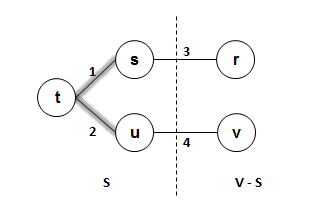
\includegraphics[width=0.5\textwidth]{q8-04.png}
\captionof{figure}{Exemplo de grafo com uma única MST com pesos nas arestas diferentes.}
\label{fig:8.4-1}
\end{center}

O corte $(S, V - S)$ respeita $A$. $(u, v)$ é uma aresta que atravessa o corte $(S, V - S)$ e é segura para $A$, ou seja, $A \cup \{(u, v)\} \subseteq T$, porém, não é de custo mínimo (\textit{light edge}).

\noindent\textbf{5. (CRLS 23.1-3)} Prove ou desprove a seguinte afirmação: Se uma aresta está contida em alguma MST, então tem peso mínimo dentre todas as arestas de algum corte no grafo.\\[6pt]
\textbf{Resposta:} Seja $T$ uma MST que contém a aresta $(u, v)$. Se tirarmos $(u, v)$ da árvore, teremos um corte $(S, V - S)$ que particiona os vértices em dois conjuntos disjuntos $S$ e $V - S$. A aresta $(u, v)$ atravessa esse corte e ela é uma aresta de custo mínimo pois, do contrário, outra aresta de custo menor poderia ser adicionada em $T$ substituindo $(u, v)$, o que produziria uma outra MST $T'$, onde $w(T') < w(T)$, contradizendo o fato de que $T$ é uma MST.

Portanto, $(u, v)$ é uma aresta de custo mínimo para o corte $(S, V - S)$.\\[6pt]

\noindent\textbf{5.1. (CLRS 23.1-4)} Dê um exemplo simples de um grafo tal que o conjunto de arestas \{$(u, v)$ : existe um corte $(S, V - S)$ tal que $(u, v)$ é uma aresta de custo mínimo atravessando o corte\} não forma uma MST.\\[6pt]
\textbf{Resposta:} Basta pensarmos em um triângulo com 3 vértices conectados por arestas de mesmo peso $w(e_1) = w(e_2) = w(e_3)$. Independente do corte, nós sempre teremos uma aresta de custo mínimo que não estará na MST pois, do contrário, teríamos um ciclo.

\begin{center}
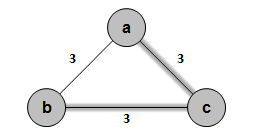
\includegraphics[width=0.35\textwidth]{q8-05-1.png}
\captionof{figure}{Exemplo de grafo onde uma aresta de custo mínimo  não pertence à MST.}
\label{fig:8.5-1-1}
\end{center}

\noindent\textbf{6. (CRLS 23.1-7)} Prove que se todos os pesos nas arestas são positivos, então qualquer subconjunto de arestas que conectam todos os vértices e tem peso total mínimo forma uma árvore. A propriedade vale se alguns pesos são negativos?\\[6pt]
\textbf{Resposta:}


\noindent\textbf{7.} Seja $T$ uma MST de um grafo com pesos positivos e distintos nas arestas. Suponha que substituímos cada peso pelo seu quadrado. Verdadeiro ou falso: $T$ ainda é uma MST para o novo grafo.\\[6pt]
\textbf{Resposta:} Verdadeiro. Substituir os pesos das arestas em um grafo ponderado $G$ pelo quadrado dos mesmos não muda a MST $T$ do grafo.

\textbf{Prova por contradição:}\\
Vamos assumir que a alteração dos pesos $w$ muda a MST $T$ de $G$ para uma outra $T'$ em $G'$, já que pelo menos uma aresta, digamos $e$, de $T$ deve ser substituída por uma outra $e'$ na nova árvore $T'$ de $G'$ com $w^2$. Isso implica que $w(e) < w(e')$ e $w^2(e) \geq w^2(e')$, o que é uma contradição.\\[6pt]

\noindent \textbf{8}. Dado um grafo conexo $G$, dizemos que duas $MSTs T$  e $T'$ são vizinhas se $T$ contém exatamente uma aresta que não está em $T'$, e $T'$ contém exatamente uma aresta que não está em $T$. Vamos construir um novo grafo (muito grande) $\mathcal{H}$ como segue. Os vértices de $\mathcal{H}$ são as $MSTs$ de $G$, e existe uma aresta entre dois vértices em $\mathcal{H}$ se os correspondentes $MSTs$ são vizinhas. É verdade que $\mathcal{H}$ sempre conexo? Prove ou dê um contra-exemplo
\\[6pt]
\noindent \textbf{Resposta:} Seja $G$ um grafo e $\mathcal{H}$ o grafo que tem como vértices todas $MSTs$ de $G$ e dois vértices de $\mathcal{H}$ são adjacentes se e somente se as $MSTs$ que eles representam são vizinhas. Queremos provar que $\mathcal{H}$ é conexo.
\\[6pt]
\noindent Se para qualquer par de $MSTs$ $T$ e $T'$ de $G$, as árvores são vizinhas então não temos nada a provar, $\mathcal{H}$ é conexo.
\\[6pt]
\noindent Se existem $T$ e $T'$ não vizinhos então achamos um caminho de $T$ a $T'$ em $\mathcal{H}$ da seguinte forma.
\\[6pt]
\noindent Sabemos que uma árvore tem $n-1$ vértices para $n = |V(G)|$ e se inserimos uma aresta a mais nessa árvore geraremos um ciclo, então podemos montar um caminho de $T$ a $T'$ em $\mathcal{H}$, inserindo uma aresta $e'$ em $T$ tal que $e' \in E(T'), e' \notin E(T)$ e $e' \in E(G)$ formando assim um ciclo em $T$ então removemos uma aresta $e$ desse ciclo em $T$, tal que $e \in E(T), e \notin E(T')$ e $e \in E(G)$, gerando assim uma $MST$ $T''$ mais parecida com $T'$, note que isso é possível por que tanto $e$ como $e'$ pertencem a uma $MST$ e portanto tem pesos minímos no ciclo formado. Repetindo esse processo chegaremos a uma $MST$ $T*$ que possuí apenas uma aresta diferente de $T'$, então concluírmos que $T'$ e $T*$ são vizinhas. Portanto podemos concluír que existe um caminho entre $T$ e $T'$ em $\mathcal{H}$ e como isso é verdade para todos pares de $MSTs$ $T$ e $T'$ de $\mathcal{H}$, logo concluírmos que $\mathcal{H}$ é conexo.\\[6pt]
\\[6pt]
\noindent \textbf{9}. Seja $G$ um grafo conexo com custos nas arestas. Uma aresta $e$ de $G$ é crítica se o aumento do custo de $e$ faz com que o custo de uma $MST$ de $G$ também aumente. Escreva uma função que determine todas as arestas críticas de $G$ em tempo $O(m \log n)$
\\[6pt]
\noindent \textbf{Resposta:} Seja $D_A$ a floresta representada pela estrutura de conjuntos disjuntos do algoritmo de Kruskal, e $T, T' \in D_A$ árvores mantida nessa floresta. Uma aresta $(u,v)$ tal que $u \in V(T)$ e $v \in V(T')$ é crítica se e somente se $(u,v)$ é uma $light$ $edge$ que respeita $A$ e não exista outra $light$ $edge$ que junte $T$ e $T'$ em $D_A$.
\\[6pt]
\noindent \textbf{Prova:}
\\[6pt]
\noindent $\rightarrow$ se $(u,v)$ é crítica então $(u,v)$ é uma $light$ $edge$ e não existe nenhuma outra $light$ $edge$ que junte $T$ e $T'$ em $D_A$.
\\[6pt] 
\noindent Verdade por que caso existisse outra $light$ $edge$ $(u',v')$ então poderiamos utiliza-la mantendo o mesmo peso da $MST$ independente do peso de $(u,v)$, ou seja, poderiamos aumentar o peso de $(u,v)$ sem aumentar o peso de uma $MST$ de $G$.
\\[6pt]
\noindent $\leftarrow$ se $(u,v)$ é a única $light$ $edge$ que junta as árvores $T$ e $T'$ então $(u,v)$ é uma aresta crítica.
\\[6pt]
\noindent Trivialmente verdade, já que para montar uma $MST$ precisamos utilizar $(u,v)$ então se aumentarmos o peso de $(u,v)$ ou escolhermos outra aresta $(u', v')$ aumentaremos o peso de qualquer $MST$ de $G$, já que $(u', v')$ tem peso maior que $(u, v)$ já que por hipótese $(u,v)$ é a única $light$ $edge$ que junta $T$ e $T'$.
\\[6pt]
\noindent Portanto ao juntar dois componentes no algoritmo de Kruskal podemos ver se a aresta é crítica ou não conforme algoritmo $\proc{Critical-Kruskal}$.

\begin{codebox}
 \Procname{$\proc{Critical-Kruskal}(G)$}
 \li $l \gets NIL, A \gets \emptyset, C \gets \emptyset$
 \li ordene as arestas de $E(G)$ em ordem crescente de peso $w_e$
 \li \For each $v \in V(G)$
 \li \Do
	$\proc{Make-Set}(v)$
      \End
 \li \For each $uv \in E(G)$ in the sorted edges
 \li \Do
 	\If $\proc{Find-Set}(u) \neq \proc{Find-Set}(v)$
 \li	\Then
 	    $A \gets A \bigcup \{uv\}$
 \li	    $\proc{Union}(uv)$
 \li	    \If $l \neq NIL$
 \li	    \Then
 	       $C \gets C \bigcup \{l\}$
 	    \End
 \li	    $l \gets uv$
 \li	    $l \gets uv$
 	 \Else
 \li	    \If $l \neq NIL$ and $w(l) = w(uv)$
 \li	    \Then
 	      $l \gets NIL$
 	    \End
         \End
     \End 
 \li \Return $C$
\end{codebox}

\noindent O algoritmo mantém a mesma estrutura de dados do que o Kruskal a linha 6, acha se a aresta sendo analisada estão na mesma árvore se sim, junta e guarda a aresta anterior é $light$ $edge$ que junta $uv$ (já que as arestas estão ordenadas), caso contrário se a aresta não junta dois componentes e tem o mesmo peso então a aresta $l$ não é crítica e recebe $NIL$, para não ser inclusa em $C$.\\[6pt]

\noindent\textbf{10.} Mostre que depois de cada execução da linha 12 do algoritmo de Prim tem-se $key[u] < \infty$.\\[6pt]
\textbf{Resposta:} Note que antes do \textit{while} da linha 6, todo vértice $u \in Q$ e $key[u] = \infty$, exceto o vértice $r$ pelo qual iniciamos a busca, onde $key[r] = key[u] = 0$. Trivialmente, $key[r] = key[u] < \infty$. Portanto, $r \in V-Q$ e isso nos dá um corte no grafo.

O \textit{loop} das linhas 8-11 atualiza $key[v]$ para todo $v \in Adj[u]$ que ainda está em $Q$. Como inicilizamos $key$ com infinito, ele será atualizado pelo menos uma vez. Logo, a fila de prioridade será reorganizada e o vértice cujo $key$ tiver o menor custo $w(u, v)$ será o novo $u$ na próxima iteração. Isso faz com que os vértices em $Q$ recebendo arestas do corte oriundas do conjunto $V - Q$ sempre tenham $key < \infty$. Como o \textit{loop} é feito até que $Q = \emptyset$, ao final teremos $key[u] < \infty$ para todo $u \in V[G]$.

\begin{center}
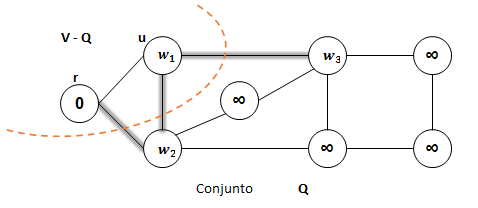
\includegraphics[width=0.6\textwidth]{q8-10.png}
\captionof{figure}{Exemplo de corte no grafo mostrando que o atributo $key[v] < \infty$ para os vértices adjacentes a $u$. As arestas sombreadas são aquelas atravessando o corte.}
\label{fig:8.10-1}
\end{center}
\\[6pt]
\textbf{11. } Suponha que temos um grafo $G$ com pesos nas arestas. Verdadeiro ou falso: Para qualquer $MST$ $T$ de $G$, existe uma execução válida do algoritmo de Kruskal que produz $T$ como saída? Dê uma prova ou um contra-exemplo.
\\[6pt]
\noindent \textbf{Resposta: }Verdadeiro. Vamos assumir por contradição que existe uma $MST$ $T'$ que nunca será gerada por uma execução do algoritmo de Kruskal. Então existe uma aresta $(u,v) \in E(T')$ que liga dois conjuntos da estrutura $\proc{UnionFind}$ $D_A$ mantida pelo algoritmo de Kruskal. Então devemos analisar 2 casos.
\begin{enumerate}
 \item Se $(u,v)$ é uma aresta de peso minímo que liga o conjunto que contém $u$ com o conjunto que contém $v$ então existe uma ordenação em que o algoritmo de Kruskal gera uma $MST$ que a contém 
 \item Se $(u,v)$ não possuí peso minímo entre todas as arestas que ligam o conjunto que contém $u$ com o conjunto que contém $v$, então podemos diminuir o peso de $T'$ escolhendo uma aresta de menor peso. Que é uma contradição já que $T'$ não é uma $MST$.
\end{enumerate}

\noindent Note que isso é verdade para qualquer aresta $(u,v)$, portanto $T'$ não existe. Que é uma contradição. Logo podemos concluir que o algoritmo de Kruskal pode gerar qualquer árvore geradora miníma de um grafo. 
\\[6pt]
\noindent \textbf{13 (CLRS Ex. 23.2-4,5)} Suponha que todos os pesos num grafo com $n$ vértices são inteiros no intervalo de 1 até $n$. Descreva como otimizar os algoritmos de Kruskal e Prim nesta situação. O que acontence se pos pesos são intervalo de 1 até $W$? 
\\[6pt]
\noindent \textbf{Resposta: } Para o algoritmo de Kruskal utilizando a estrutura de conjuntos disjuntos utilizando $\proc{Union-By-Rank}$ e compressão de caminhos o tempo gasto assintoticamente é definido pela ordenação de arestas, no começo do algoritmo, se sabemos que o peso máximo das arestas é $n$, então podemos usar o $\proc{Counting-Sort}$ e diminuir o tempo de $O(m \lg n)$ para $O(m + n)$, já que o laço abaixo da ordenação gasta tempo linear, se o peso máximo é $W$ então utilizando o $\proc{Counting-Sort}$ o algoritmo de Kruskal gastará tempo $O(m + W)$. Como o algoritmo de Prim utiliza uma fila de prioridades que normalmente é implementada como uma min-heap não é possível melhorar o tempo assintotico do algoritmo.

\indent\textbf{15.} O diâmetro de um grafo é o máximo das distâncias entre dois vértices. Escreva código que usa o algoritmo de Dijkstra para calcular o diâmetro de um grafo.\\[6pt]
\textbf{Resposta:} Para calcular o diâmetro de um grafo $G$ podemos aplicar o \proc{Dijkstra} usando cada vértice $v \in V[G]$ como fonte da busca, retornando o maior valor de $d$ para cada busca. A maior distância será, então, o diâmetro de $G$.

\begin{codebox}
\Procname{$\proc{Graph-Diameter}(G, w)$}
\li $diameter \gets 0$
\li \For each $u \in V[G]$
\li \Do
        $max\_d = \proc{Dijkstra-Diameter}(G, w, u)$
\li     \If $max\_d > diameter$
\li     \Then 
            $diameter \gets max\_d$
        \End
    \End
\li \Return $diameter$
\end{codebox}

\begin{codebox}
\Procname{$\proc{Dijkstra-Diameter}(G, w, s)$}
\li $\proc{Initialize-Single-Source}(G, s)$
\li $S \gets \emptyset$
\li $Q \gets V[G]$
\li \While $Q \neq \emptyset$
\li \Do
        $u \gets \proc{Extract-Min}(Q)$
\li     $S \gets S \cup \{u\}$
\li     \For each $v \in Adj[u]$
\li     \Do
            $\proc{Relax}(u, v, w)$
        \End
    \End
\li \Return $u.\id{d}$ \Comment the last $u$ removed from $Q$
\end{codebox}

\textbf{Consumo de Tempo:} A inclusão da linha 9 no \proc{Dijkstra-Diameter} não muda o consumo de tempo do \proc{Dijkstra}, que continua $O(V lg E)$. Como executamos uma vez para cada vértice no \textit{loop} da linha 2 da rotina $\proc{Graph-Diameter}$, temos que o tempo total será $O(V(V lg E))$.\\[6pt]

\noindent\textbf{16.} Considere um dígrafo (grafo orientado) com custos positivos associados aos vértices. O custo de um caminho num tal dígrafo é a soma dos custos dos vértices do caminho. Queremos encontrar um caminho de custo mínimo dentre os que começam num vértice $s$ e terminam num vértice $t$. Adapte o algoritmo de Dijkstra para resolver esse problema.\\[6pt]
\textbf{Resposta:} Basta pararmos o algoritmo de Dijkstra quando o vértice $t$ for encontrado. Como a estratégia do algoritmo é gulosa, ao retirarmos o vértice $t$ da fila de prioridade, já teremos o caminho mínimo de $s$ a $t$.

\begin{codebox}
\Procname{$\proc{Dijkstra-Single-Pair}(G, w, s, t)$}
\li $\proc{Initialize-Single-Source}(G, s)$
\li $S \gets \emptyset$
\li $Q \gets V[G]$
\li \While $Q \neq \emptyset$
\li \Do
        $u \gets \proc{Extract-Min}(Q)$
\li     $S \gets S \cup \{u\}$
\li     \If $u == t$
\li     \Then
            \Return
        \End
\li     \For each $v \in Adj[u]$
\li     \Do
            $\proc{Relax}(u, v, w)$
        \End
    \End
\end{codebox}

\textbf{Consumo de Tempo:} A inclusão das linhas 7-8 não muda o comportamento assintótico original do \proc{Dijkstra}, que continua que continua $O(E lg V)$.\\[6pt]

\noindent\textbf{18. (CLRS 24.3-2)} Mostre que o algoritmo de Dijkstra pode produzir resultados errados se o dígrafo tiver arcos de custo estritamente negativo.\\[6pt]
\textbf{Resposta:} Um exemplo para dígrafos pode ser visto na figura \ref{fig:8.18-1}.

\begin{center}
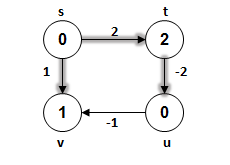
\includegraphics[width=0.35\textwidth]{q8-18.png}
\captionof{figure}{Dígrafo com arcos estritamente negativos.}
\label{fig:8.18-1}
\end{center}

A execução de todas as iterações do \proc{Dijkstra} produz o caminho mínimo destacado pelas arestas sombreadas. O valor de $d[v]$ está errado, pois existe um caminho mínimo de $s \leadsto v$ de custo menor que 1, por exemplo, o caminho $p' = s \leadsto t \leadsto u \leadsto v$, onde $w(p') = -1 < 1$.\\[12pt]

\noindent\textbf{21. (CLRS 24.3-3)} Suponha que trocamos a linha 4 do algoritmo do Dijkstra como segue
\begin{center}
4. $while|Q| > 1$
\end{center}
Isso faz com que a execução do laço execute $|V| - 1$ vezes no lugar de $|V|$ vezes. Será que o algoritmo continua correto?\\[6pt]
\textbf{Resposta:} Sim, o algoritmo continua funcionando. Seja $u$ o vértice restante que não é extraído da fila de prioridades $Q$. Se $u$ não é alcançável de $s$, então $d[u] = \delta(s, u) = \infty$. Se $u$ é alcançável de $s$, existe um caminho mínimo $p = s \leadsto x \rightarrow u$.

Quando o vértice $x$ foi extraído de $Q$, $d[x] = \delta(s, x)$ e, então, a aresta $(x, u)$ já foi "relaxada" e, portanto, $d[u] = \delta(s, u)$.\\[6pt]
\clearpage

\begin{center} 
\textbf{\large{Lista 9}}
\end{center}

\noindent\textbf{1.} Defina \textit{algoritmo eficiente}. Defina \textit{problema de decisão}. Defina \textit{verificador polinomial} para \const{sim}. Defina \textit{verificador polinomial} para \const{não}. Defina as classes P, NP e coNP. Dê um exemplo de um problema em cada uma dessas classes, justificando a sua pertinência à classe.\\[6pt]
\textbf{Resposta:}

\textit{Algoritmo eficiente:} um algoritmo é eficiente se ele resolve um dado problema em tempo polinomial, ou seja, se o seu consumo de tempo no pior caso é limitado por um polinômio no tamanho das instâncias do problema. Em outras palavras, o algoritmo é polinomial se ele resolve o problema em tempo $O(n^k)$ para alguma constante $k$.\\

\textit{Problema de decisão:} aquele cuja solução é uma resposta do tipo \const{sim}/\const{não}.\\

\textit{Verificador polinomial} para \const{sim} a um problema $\pi$ é um algoritmo polinomial $A$ tal que\\
\textbf{1.} para qualquer instância $X$ de $\pi$ com resposta \const{sim}, existe um $Y$ em $\Sigma^\star$, tal que $A(X, Y)$ devolve \const{sim}\\
\textbf{2.} para qualquer instância $X$ de $\pi$ com resposta \const{não}, existe um $Y$ em $\Sigma^\star$, tal que $A(X, Y)$ devolve \const{não}\\
\textbf{3.} $A$ consome tempo polinomial em $|X|$\\

\textit{Verificador polinomial} para \const{não} a um problema $\pi$ é um algoritmo polinomial $A$ tal que\\
\textbf{1.} para qualquer instância $X$ de $\pi$ com resposta \textcolor{red}{\const{não}}, existe um $Y$ em $\Sigma^\star$, tal que $A(X, Y)$ devolve \const{sim}\\
\textbf{2.} para qualquer instância $X$ de $\pi$ com resposta \textcolor{red}{\const{sim}}, existe um $Y$ em $\Sigma^\star$, tal que $A(X, Y)$ devolve \const{não}\\
\textbf{3.} $A$ consome tempo polinomial em $|X|$

Onde $Y$ é um certificado para \const{sim}/\const{não} da instância $X$ de $\pi$.\\

\textit{Classe P:} conjunto dos problemas de decisão tratáveis, isto é, que são solúveis em tempo polinomial.
\textbf{Exemplo:} problema da mochila fracionária está em $P$, já que pode ser resolvido em tempo $O(n lg n)$.\\

\textit{Classe NP:} conjunto dos problemas de decisão que possuem um verificador polinomial para a resposta \const{sim}, ou seja, se existe um algoritmo que, ao receber uma instância $X$ de $\pi$ e uma suposta solução $S$ de $X$, responde \const{sim} ou \const{não} conforme $S$ seja ou não solução de $X$,  e  consome tempo limitado por um polinômio no tamanho de $X$ para responder \const{sim}. \textbf{Exemplo:} O problema do ciclo hamiltoniano está em NP, pois é possível verificar em tempo polinomial se uma dada permutação dos vértices é um ciclo do grafo.\\

\textit{Classe coNP:} consiste nos problemas de decisão que são complementos de problemas de decisão em NP, ou seja, problemas para os quais existe um certificado (curto) para a resposta \const{não}. \textbf{Exemplo:} O problema do quadrado perfeito está em coNP,  pois é possível verificar em tempo polinomial se um certo número natural $n$ \textbf{não} é um quadrado perfeito. Em outras palavras, basta exibir um número natural $k$ tal que $k^2 < n < (k+1)^2$.  Um tal $k$ é um certificado de que $n$ não é um quadrado perfeito.\\[6pt]

\noindent\textbf{2.} Mostre que SAT está em NP. (Essa é a parte fácil do teorema de Cook.)\\[6pt]
\textcolor{red}{\textbf{Resposta:}} Para mostrar que o SAT está em NP, temos que mostrar que existe um algoritmo $A(C,X,Y)$ que verifica o certificado $Y$ que devolve SIM se $Y$ pertence ao conjuto de soluções para a instância $C, X$.

Seja $C$ um conjunto de clasulas sobre um conjunto de variáveis $X$, então 
podemos considerar $C$ e $X$  nossa instância do problema SAT. Seja $Y$ uma 
atribuição das variáveis de $X$, podemos considerar $Y$ como nosso certificado, 
já que se as clasulas $C$ forem satisfazivel por $Y$ então a formula é 
satisfazivel. É fácil notar que podemos escrever um algoritmo que leia $X,C$ e 
$Y$ e imprime SIM se e somente se $Y$ satisfaz $C$, álem disso esse algoritmo 
pode ser implementado de forma a consumir tempo polinomial em $|X|$ e $|C|$, 
(note que $|Y| = |X|$). Portanto SAT pode ser verificado e certificado em tempo 
polinomial, logo SAT está em NP.\\[6pt]

\noindent\textbf{3.} Uma coleção $C$ de cláusulas sobre um conjunto $X$ de variáveis booleanas é uma tautologia se toda atribuição a $X$ satisfaz $C$. O problema \proc{tautologia} consiste em, dado $X$ e $C$, decidir se $C$ é ou não uma tautologia. O problema \proc{tautologia} está em NP? Está em coNP? Justifique suas respostas.\\[6pt]
\textcolor{red}{\textbf{Resposta:}}

\noindent\textbf{4.} O problema \proc{2-sat} consiste na restrição de \proc{sat} a instâncias $X$ e $C$ em que toda cláusula de $C$ tem exatamente dois literais. Mostre que o \proc{2-sat} está em P, ou seja, descreva um algoritmo polinomial que resolva o \proc{2-sat}.\\[6pt]
\textcolor{red}{\textbf{Resposta:}}

\noindent\textbf{5.} Mostre que \proc{2-coloração} está em P.\\[6pt]
\textcolor{red}{\textbf{Resposta:}}

\noindent\textbf{6.} Seja $G = (V, E)$ um grafo. Um conjunto $S \subseteq V$ é independente se quaisquer dois vértices de $S$ não são adjacentes. Ou seja, não há nenhuma aresta do grafo com as duas pontas em $S$. O problema
IS consiste no seguinte: dado um grafo $G$ e um inteiro $k \geq 0$, existe um conjunto independente em $G$ com $k$ vértices? Mostre que IS é NP-completo.\\[6pt]
\textcolor{red}{\textbf{Resposta:}} Para mostrar o problema de decidir é NP-completo precisamos mostrar que o problema é NP e que podemos reduzir um problema NP-completo a o problema que estamos querendo mostrar que é NP.

Seja $G = (V, E)$ um grafo e $k$ um número inteiro maior que zero e $S$ um subconjunto de $V(G)$ com $k$ vértices. Tomando $G$ e $k$ como uma instância do problema do conjunto independente e $S$ um certificado. Podemos verificar se $G$ tem um conjunto independente de $k$ vértices verificando se nenhum par de vértices em $S$ são adjacentes. É fácil notar que podemos escrever um algoritmo que faz essa verificação é devolve sim quando $S$ é um conjunto independente e NÃO caso contrário. Ademais esse algoritmo gasta tempo polinomial em $|G|$. portanto o problema de conjunto independente está em NP.

Vamos mostrar que o problema de conjunto independente é NP-completo fazendo a redução polinomial: Conjunto independente $\leq_P$ Clique em grafo. Para isso vamos utilizar o grafo complementado $\bar{G}$, um grafo complementado $\bar{G}$ de um grafo $G$ é o grafo formado pelos vértices do grafo $G$ e existe uma aresta $(v,u)$ em $\bar{G}$ se e somente se $(u,v)$ não são adjacentes em $G$. Disso tiramos o seguinte lema.

\begin{lemma}
 \: um grafo $G$ tem um clique de tamanho $k$ se e somente se seu grafo complementado $\bar{G}$ tem um conjunto independente de tamanho $k$
\end{lemma}

\textbf{Prova}: Pela definição, $e$ é uma aresta de $G$ se e somente se $e$ não é uma aresta de $\bar{G}$. Se temos um clique de tamanho $k$ em $G$, então temos que existem $k$ vértices em $G$ que estão conectados entre si por um conjunto de arestas $C$ o grafo complementado $\bar{G}$ não tem essas arestas então portanto esses mesmos vértices formam um conjunto independente em $\bar{G}$ de tamanho $k$. Similarmente podemos provar que o conjunto independente em $\bar{G}$ é um clique em $G$.

É fácil notar que podemos escrever um algoritmo que transforma $G$ em $\bar{G}$ pegando os seus vértices e adicionando as arestas necessárioas quando essa aresta não está em $G$. É fácil notar também que isso pode ser feito em um algoritmo que consome tempo polinomial. Conforme visto em aula, decidir se um grafo possuí um clique de tamanho $k$ é NP-dificil logo com essa redução polinomial mostramos que decidir se o grafo possuí um conjunto independente de $k$ vértices também é NP-dificil. \\[6pt]


\noindent\textbf{7.} Seja $G = (V, E)$ um grafo. Uma \proc{3-coloração} de $G$ é uma função $c : V \rightarrow {1, 2, 3}$ tal que $c(u) \neq c(v)$, para toda aresta $uv \in E$. Considere o

\indent\textbf{Problema} \proc{3-coloração}: Dado um grafo, determinar se ele tem ou não uma \proc{3-coloração}.

Mostre que o \proc{3-coloração} está em NP.\\[6pt]
\textcolor{red}{\textbf{Resposta:}}

\noindent\textbf{8.} Mostre que o problema abaixo é NP-completo.

\indent\textbf{Problema} \proc{partição}: Dada uma coleção $S$ de números, decidir se existe uma sub-coleção $S'$ de $S$ cuja soma é igual a soma dos números em $S \ S'$, ou seja,
\begin{center}
$\sum_{x \in S}{x} = \sum_{x \notin S}{x}$
\end{center}
\textcolor{red}{\textbf{Resposta:}}

\noindent\textbf{9.} Mostre que o problema abaixo é NP-completo.

\indent\textbf{Problema} \proc{mochila}: Dado um número $W$, um número $V$, um número inteiro positivo $n$, uma coleção de números $w_1, \ldots , w_n$, e uma coleção de números $v_1, \ldots , v_n$, decidir se existe um subconjunto $S$ de $\{1, \ldots , n\}$ tal que

\begin{center}
$\sum_{i \in S}{w_i} \leq W$ e $\sum_{i \in S}{v_i} \geq V$
\end{center}
\textcolor{red}{\textbf{Resposta:}}
\clearpage

\begin{center}
\textbf{\large{CLRS (Outros)}}
\end{center}

\noindent A.1-7 Avalie o produtório $\prod_{k=1}^n 2(4^k)$.\\[6pt]
\begin{align*}
\prod_{k=1}^n 2(4^k) = \prod_{k=1}^n 2({(2^2)}^k) = \prod_{k=1}^n 2(2^{2k}) = \prod_{k=1}^n 2^{2k + 1}
\end{align*}

Se avaliarmos o produtório para $n = 3$, por exemplo:
\begin{align*}
\prod_{k=1}^n 2^{2k + 1} = 2^{2 + 1} \times 2^{4 + 1} \times 2^{6 + 1}
\end{align*}

Percebemos que o expoente de 2 cresce em uma série aritmética:
\begin{align*}
\sum_{k=1}^n 2k + 1 = \sum_{k=1}^n 2k + \sum_{k=1}^n 1 = 2\sum_{k=1}^n k + n =
2(\frac{n(n + 1)}{2}) + n = n(n + 2)
\end{align*}

Portanto:
\begin{align*}
\prod_{k=1}^n 2(4^k) = 2^{n(n + 2)}
\end{align*}
\end{document}
